\section{Исследование и построение решения задачи}
\label{sec:Chapter3} \index{Chapter3}

\subsection{План решения и разбитие на подзадачи}

Напомню, что для достижения цели я поставил перед собой следующие задачи:
\begin{enumerate}
    \item Определить, какой формат представления CAD объекта лучше.
    \item На предпочтительном формате внедрить изменения в train-данные, которые повысят метрики эксперимента.
\end{enumerate}

\paragraph{Зачем тестировать различные форматы.}
На данный момент не существует исследований, которые сравнивали результаты генерации на различных кодовых представлениях \textit{constructive-sequence}.
Однако, хотя логика построения геометрии в каждом формате должна быть одинаковой, синтаксис и структура кода могут приводить к различиям в работе.
Кроме того, в зависимости от способа представления меняется длина кода.
Введение дополнительных переменных способно дать определённые преимущества при реализации 3D-операций, требующих селекторов,
но может привести к ухудшению некоторых метрик и потере способности к реализации других операций.

Поиск «золотой середины», при которой кодовое представление обладает достаточной функциональностью и при этом остаётся коротким и синтаксически понятным, — важная задача в генерации CAD-объектов.

\subsection{CADAxt — универсальный формат хранения CAD}
Для начала отметим, что при тестировании различных представлений для CAD-моделей
хочется реализовать промежуточный этап хранения данных. Это позволит впоследствии
добавлять новые форматы представления при необходимости. Подобная идея также
возникает из необходимости иметь реальные данные, получаемые путём парсинга публичных сайтов.

Таким образом, данный формат должен быть гибким для добавления дополнительных параметров и операций,
в то время как поддержание их перевода в нужные форматы остаётся на этапе формирования датасета.

Подобную идею уже реализовали авторы статьи \textit{DeepCAD}. В~ней они распарсили данные с сайта Onshape в определённый формат JSON,
структура которого была заимствована из датасета Fusion360.
Их формат поддерживает только две операции: \texttt{Sketch} и \texttt{Extrude}.

Для внедрения других типов операций была внедрена ссылочная система на топологию, созданную при применении операции.
Она необходима и является универсальным селектором для операций, требующих выбора топологии, например:
\texttt{Fillet} (сглаживание ребра), \texttt{Chamfer} (срезка ребра).

Формат, описывающий \textit{constructive sequence}, получил название \texttt{CADAxt}
и оформлен в виде библиотеки, доступной по ссылке: \href{https://github.com/axtonio/cadaxt}{\texttt{https://github.com/axtonio/cadaxt}}.

Однако в рамках настоящих экспериментов будут использоваться только операции \texttt{Sketch} и \texttt{Extrude}.
Для простоты изложения детали реализации ссылочной системы будут опущены здесь.
Рассмотрим на простом примере строение подобного JSON:

\begin{figure}[]
    \centering
    \begin{minipage}[]{0.4\textwidth}
        \centering
        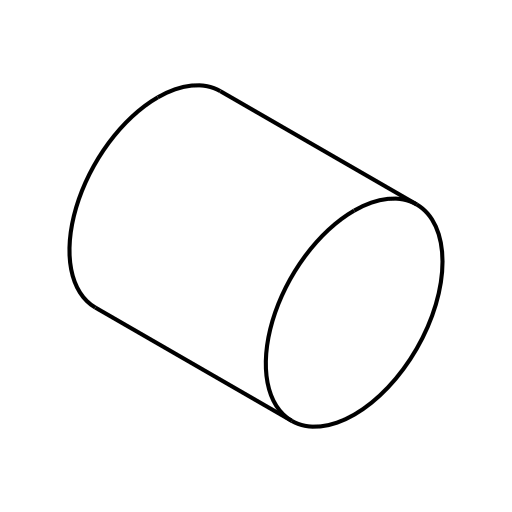
\includegraphics[width=\linewidth]{cylinder.png}
    \end{minipage}
    \hfill
    \begin{minipage}[]{0.5\textwidth}
        \centering
        \footnotesize
        \begin{verbatim}
{
  "sequence": [
    {
      "type": "Sketch",
      "entity": "sketch1_id"
    },
    {
      "type": "ExtrudeFeature",
      "entity": "extrude1_id"
    }
  ],
  "entities": {
    "sketch1_id": {
      "profiles": {
        "profile1_id": {
          "loops": [
            {
              "is_outer": true,
              "profile_curves": [
                {
                  "curve": "curve1_id",
                  "center_point": {
                    "x": 0.0,
                    "y": -50.0,
                    "z": 0.0
                  },
                  "radius": 45.0,
                  "normal": {
                    "x": 0.0,
                    "y": 1.0,
                    "z": 0.0
                  },
                  "type": "Circle3D"
                }
              ]
            }
          ]
        }
      },
      ...
    },
    "extrude1_id": {
      "reference_profiles": [
        {
          "parent": "sketch1_id",
          "id": "profile1_id"
        }
      ],
      "extent_one": {
        "distance": {
          "value": 100.0
        },
        ...
      }
    }
  }
}
\end{verbatim}
    \end{minipage}
    \caption{Представление цилиндра в формате CADAxt.}
\end{figure}

\newpage

Под ключом \texttt{sequence} идёт описание последовательности команд,
где \texttt{type}~— тип операции, а \texttt{entity}~— уникальный \texttt{id} операции.
Далее, под ключом \texttt{entities} хранится параметрическое описание каждой команды по соответствующему \texttt{id}.
Некоторые параметры здесь специально опущены, так как они не потребуются в~дальнейшем тексте.

Для понимания строения CAD-объекта обсудим параметры \texttt{Sketch}.
Каждый скетч состоит из \textit{loops} (замкнутых кривых) и \textit{profiles}.
Кривые (\texttt{curve}) бывают трёх типов: \texttt{Arc} (дуга), \texttt{Circle} (окружность) и \texttt{Line} (линия).
Безусловно, в реальном CAD-пакете есть и другие типы кривых (например, B-сплайны),
но в рамках данной работы мы ограничимся указанными тремя.
Набор \textit{Loop}, по которым можно однозначно определить ориентацию, формирует \textit{Profile}.
Валидный профиль всегда состоит из внешнего \textit{Loop} и внутренних непересекающихся,
причём внутренние задают отверстия во внешнем.

\begin{figure}[h!]
    \centering
    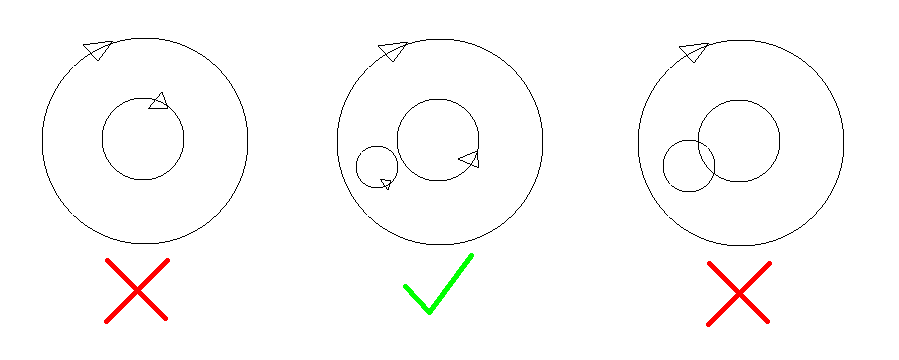
\includegraphics[width=0.7\textwidth]{sketches.png}
    \caption{Пример валидных и невалидных скетчей.}
    \label{fig:sketches}
\end{figure}

Координаты, описывающие скетч, заданы в трёхмерном пространстве относительно стандартной системы отсчёта.
Однако, по сути, скетч~— это 2D-операция, задаваемая на плоскости.
При реализации \textit{profile} может быть вычислена плоскость, относительно которой рисуется скетч,
что даёт возможность отказаться от третьей координаты и задавать скетч параметрами плоскости и координатами в~этой плоскости.
В формате CADAxt для операции \texttt{Sketch} хранится параметр \texttt{transform}, указывающий плоскость,
относительно которой рисуется скетч.

Теперь рассмотрим параметры экструдирования:
\begin{enumerate}
    \item \texttt{profiles}~— список профилей, к которым применяется экструд.
          Он однозначно задаётся путём указания \texttt{id} скетча и \texttt{id} нужного профиля.
    \item \texttt{extent\_one}~— величина, на которую выдавливается скетч по направлению его нормали.
          Направление может меняться при наличии дополнительных параметров, специально опущенных здесь.
\end{enumerate}

Таким образом, описанный формат даёт полноценное описание \textit{constructive sequence}
относительно операций \texttt{Sketch} и \texttt{Extrude}. Не рекомендуется использовать его напрямую для генерации,
так как размер подобного файла может достигать нескольких тысяч символов.
Однако он легко транслируется в любые иные форматы, что является существенным преимуществом при тестировании различных представлений.

\subsection{CADQuery и CADScript.}

После создания унифицированного формата необходимо решить три основные задачи:
\begin{enumerate}
    \item Определить, какие форматы представления CAD будут сравниваться.
    \item Определить, на каких данных будет происходить обучение.
    \item Выбрать архитектуру модели, подходящую для решения поставленной задачи.
\end{enumerate}

Отвечая на первый вопрос, на ум сразу приходят форматы \texttt{CADQuery} и \texttt{PythonOCC}.
\texttt{PythonOCC}~— это низкоуровневый способ создания CAD-объектов, основанный на технологиях OpenCascade.
Формат \texttt{CADQuery} представляет собой надстройку над \texttt{PythonOCC} и обеспечивает более удобный
способ записи. По сути, \texttt{CADQuery} является набором макросов над \texttt{PythonOCC}, благодаря чему
код одной и той же топологии получается более компактным именно в \texttt{CADQuery}. Тем не менее
сравнивать эти два формата на равных основаниях некорректно, поэтому необходимо подобрать ещё один формат,
который, с одной стороны, будет иметь более лаконичное представление, а с другой --- позволит сопоставить его
с \texttt{CADQuery}.

В литературе был предложен формат \texttt{OpenECAD}~\cite{yuan24_openecad}, в котором чётко описаны правила
оформления и представления скетчей. Основные моменты, выделяемые в \texttt{OpenECAD}, следующие:
\begin{enumerate}
    \item Моделирование в CAD обычно сводится к последовательности операций, приводящих к созданию твердотельных форм.
          В \texttt{OpenECAD} эти операции оформляются в виде структурированных команд.
    \item Скетчи в \texttt{OpenECAD} задаются на плоскости и определяются с помощью примитивов:
          линий, дуг и окружностей, а также их параметров.
    \item Для получения трёхмерных объектов в \texttt{OpenECAD} используется исключительно операция
          «скетч-экструзия», когда 2D-скетч преобразуется в 3D-форму за счёт протяжки.
    \item В \texttt{OpenECAD} применяются читаемые обозначения операций, что облегчает понимание
          и использование кода.
\end{enumerate}

\texttt{CADQuery}~— это большая библиотека с богатым набором функций и селекторов. Однако у неё есть
один недостаток: нет встроенного селектора, позволяющего выбирать рёбра, образованные конкретной
операцией (например, экструзией). Такой селектор важен при генерации последовательности действий:
если инженер в процессе проектирования видит текущее состояние 3D-модели и выбирает конкретное
ребро, плоскость или точку, то генератору необходимо отслеживать, какие элементы были созданы на предыдущих шагах.

В \texttt{OpenECAD} формат описания CAD-объектов более избыточен, однако он удобен для реализации
подобных селекторов. Из-за этой гибкости код в \texttt{OpenECAD} может получаться длиннее, чем в
\texttt{CADQuery}.

На основе подхода из \texttt{OpenECAD} был разработан формат \texttt{CADScript}. Его главное отличие
заключается в том, что он поддерживает дополнительные операции, не рассматриваемые в данной работе,
а также предусматривает квантизацию.

Примеры кода для двух представлений показаны на рисунке~\ref{fig:cadformats}.

\begin{figure}[h!]
    \centering
    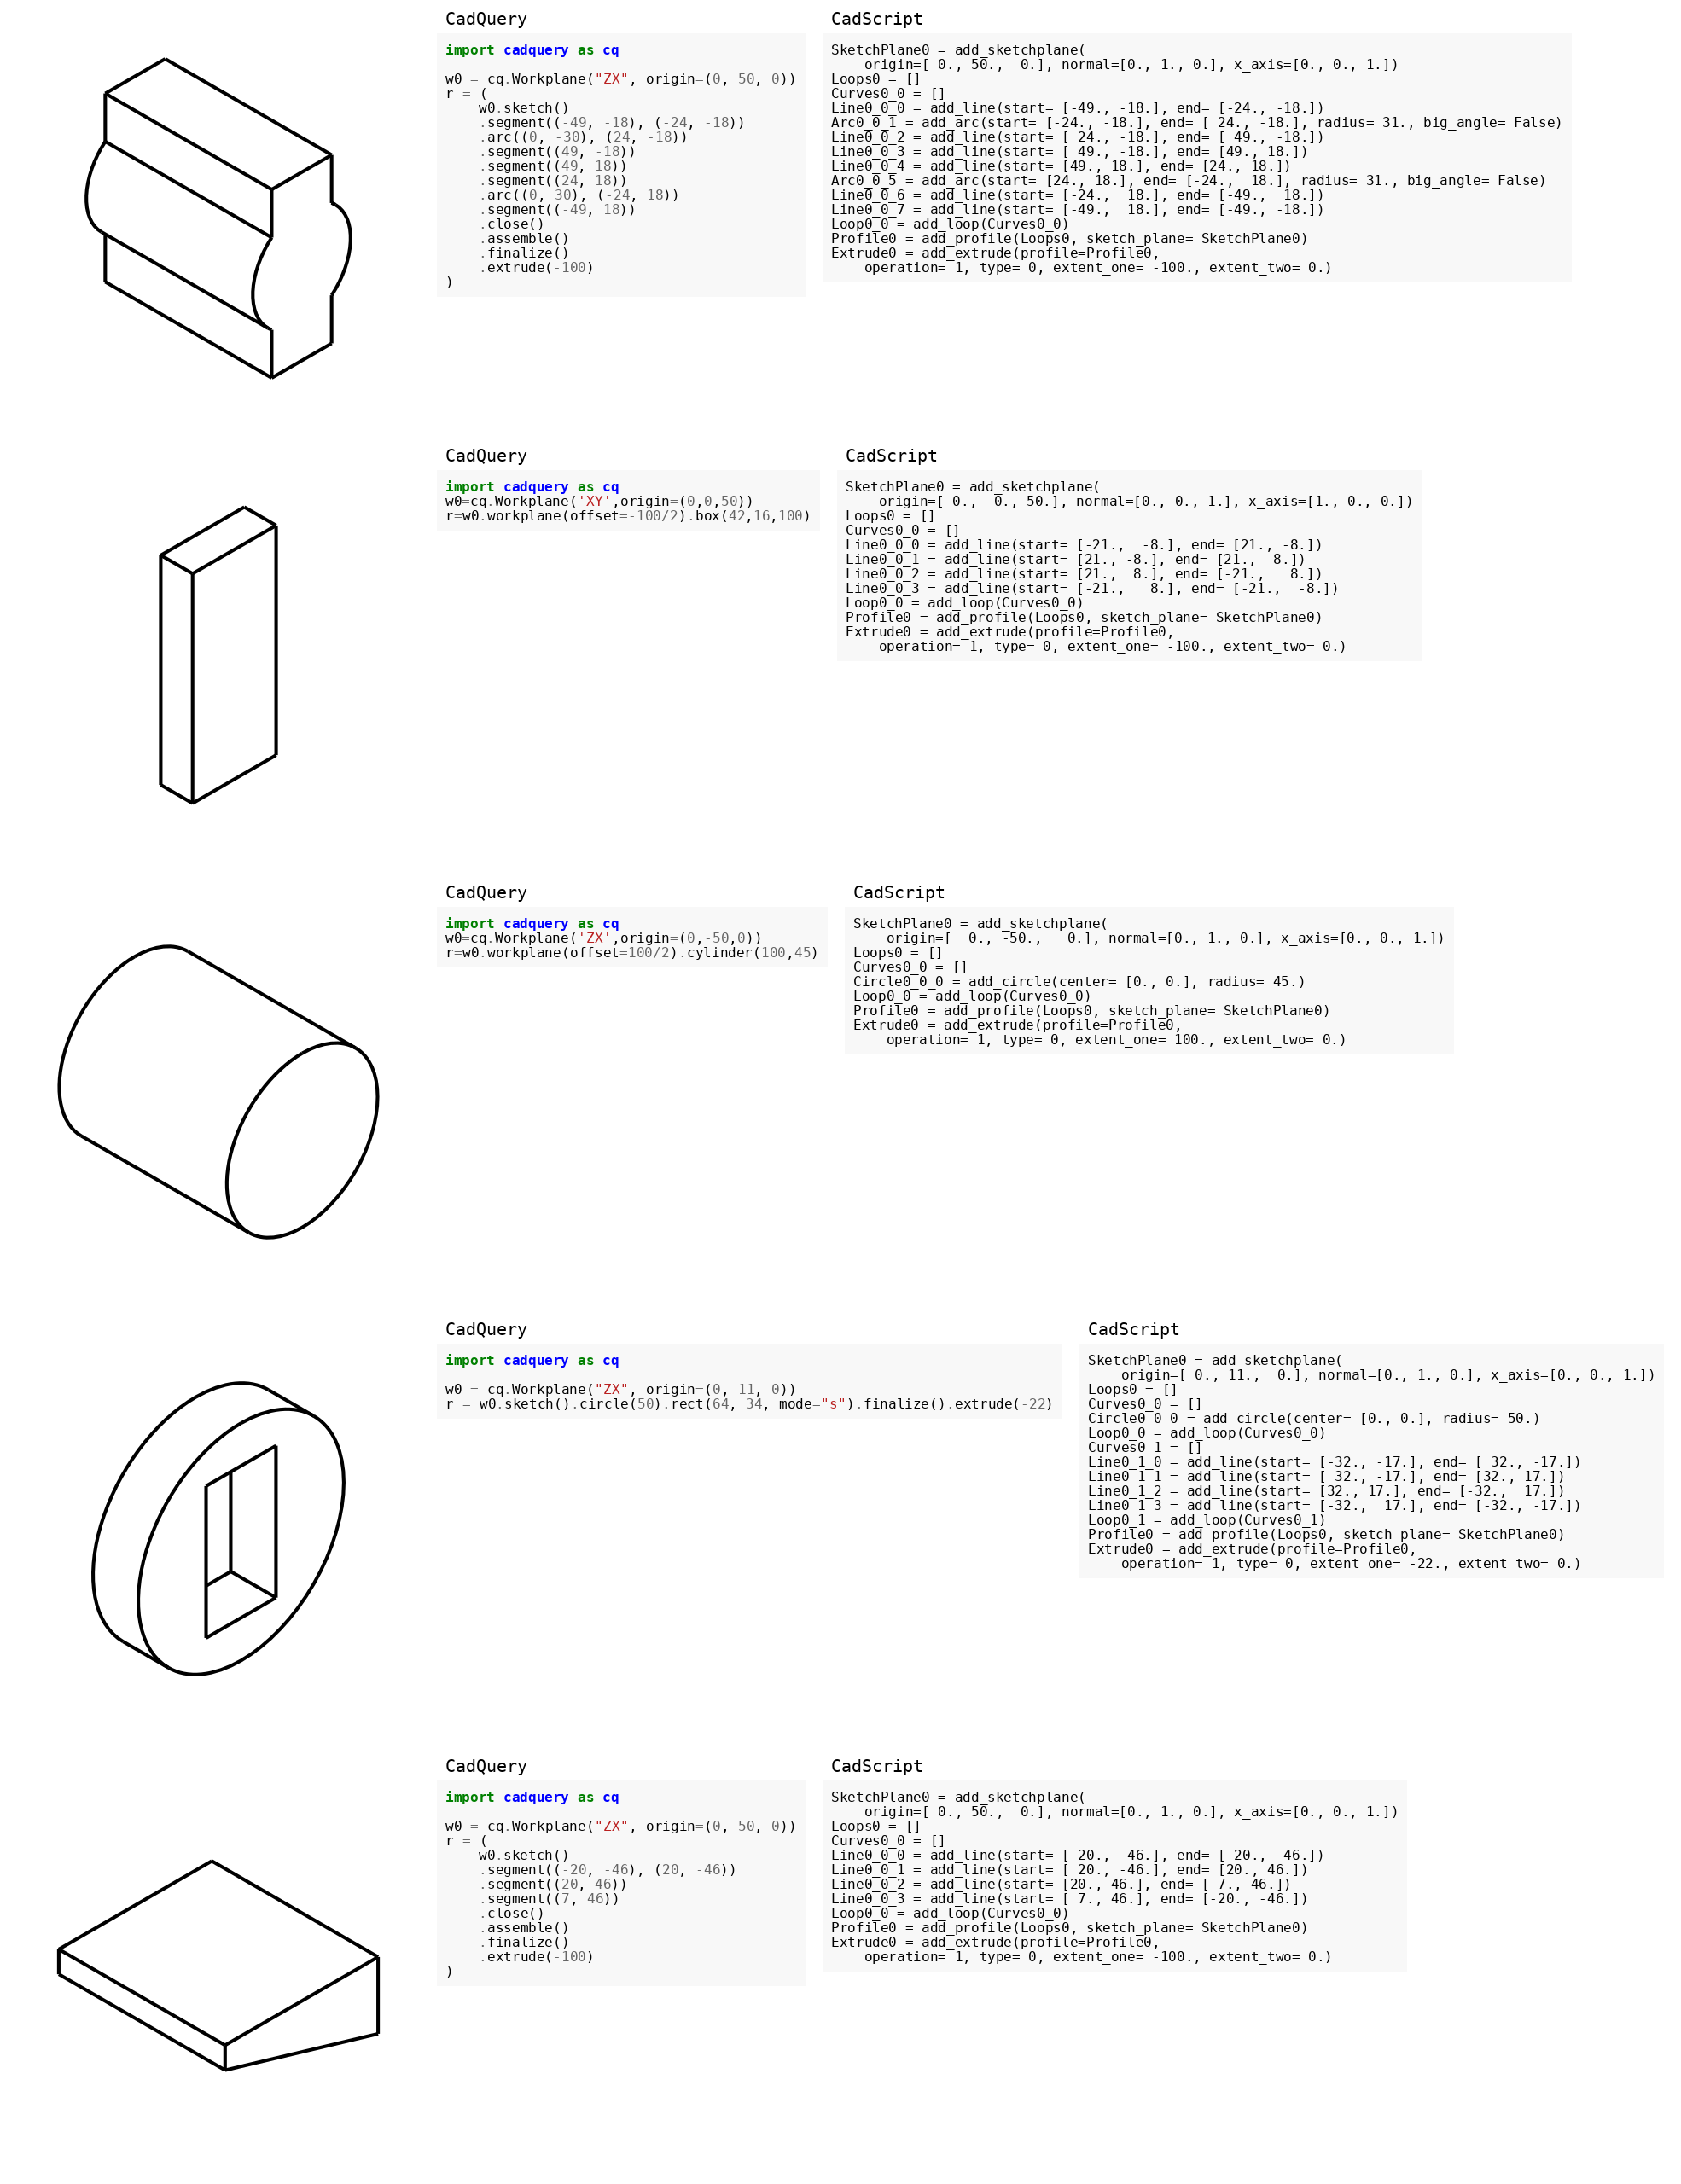
\includegraphics[width=1\textwidth]{stacked_result.png}
    \caption{Примеры представлений \texttt{CADQuery} и \texttt{CADScript}.}
    \label{fig:cadformats}
\end{figure}

\paragraph{Использование CADRecode и связка с CADAxt.}
Для решения второго и третьего вопросов в работе было выбрано решение
\texttt{CADRecode}~\cite{rukhovich24_cadrecode}. Его автор в своей статье разработал генератор синтетических
данных, которые показали лучшие результаты на бенчмарках DeepCAD и Fusion360.
Архитектура модели в \texttt{CADRecode} достаточно проста и быстро обучается,
не требуя больших вычислительных ресурсов.

В рамках настоящей работы было принято решение встроить в генератор
\texttt{CADRecode} конвейер перевода в универсальный формат \texttt{CADAxt}, из
которого затем реализован трансфер в \texttt{CADQuery} и
\texttt{CADScript}. После этого модель обучалась на одних и тех же облаках точек,
но с различными кодовыми представлениями.

Генератор одного миллиона синтетических данных работал в течение 7,5 часов на 8 H100
используя 96 CPU. То есть скорость генерации одного семпла составляет 0.4/sec на одном ядре

\subsection{Подход CAD-Recode.}

\begin{figure}[h!]
    \centering
    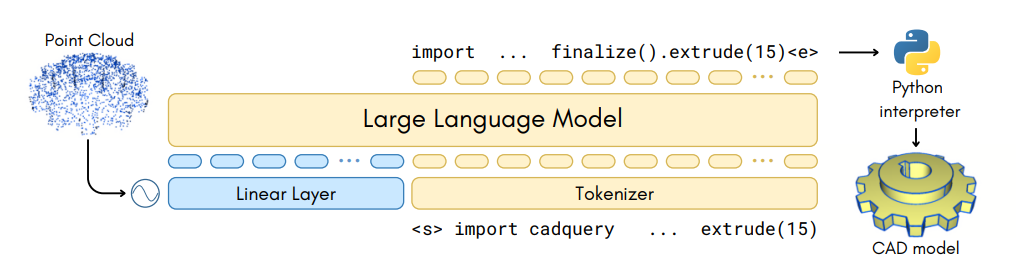
\includegraphics[width=1\textwidth]{cadrecode_arc.png}
    \caption{Архитектура CAD-Recode}
    \label{fig:cadrecode_arc}
\end{figure}

\texttt{CAD-Recode} опирается на предварительно обученных специалистов и их опыт
работы с Python-кодом, дополняя их возможностями по обработке облаков точек, а
также знаниями, специфичными для CAD-кода на Python. Как показано на рис.~4 в
оригинальной статье, архитектура \texttt{CAD-Recode} состоит из двух частей:
(1)~проектора облака точек, преобразующего 3D-облако точек в обучаемые токены, и
(2)~предварительно обученного авторегрессионного CAD-декодера на базе LLM.

\textbf{Модуль проекции облака точек.} В \texttt{CAD-Recode} представлен лёгкий
модуль проекции~$\Psi_P$, который напрямую отображает плотное облако точек
$P \in \mathbb{R}^{n \times d_p}$ (где $d_p = 3$ соответствует размерности
координат) в последовательность из $n_p$ токенов $Q_p = [q^1_p, \dots, q^{n_p}_p]
    \in \mathbb{R}^{n_p \times d_q}$, где $d_q$~--- размерность встраивания. Модуль
проекции, обучаемый совместно с модулем CAD-код-декодера, состоит из трёх простых
компонентов: (1)~алгоритма выбора самых удалённых точек для уменьшения входного
облака точек до $n_p$; (2)~позиционного кодирования координат методом Фурье;
(3)~линейного слоя, проецирующего закодированные координаты в $Q_p$.

\textbf{LLM в качестве CAD-декодера.} В качестве CAD-декодера кода, обозначаемого
$\Psi_{\text{LLM}}$, выступает предварительно обученный LLM-специалист,
приспособленный к задаче генерации кода CAD. В качестве базы берётся модель
\texttt{Qwen2-7b}. На вход этому декодеру подаются токены $Q_p$ от проектора облака точек,
дополненные кодовыми токенами $Q_t \in \mathbb{R}^{n_t \times d_q}$,
полученными после токенизации входного кода. Полная
входная последовательность обозначается $[Q_p; Q_t] \in
    \mathbb{R}^{(n_p + n_t) \times d_q}$. Модель предсказывает следующую часть
кодовой последовательности CAD, сопоставляя каждый предсказанный токен с
символом из словаря~$\Sigma$ (буквенно-цифровые символы и операторы). Таким
образом, \texttt{CAD-Recode} перенастраивает возможности моделирования LLM для
задачи преобразования облаков точек в исполняемый CAD-код.

\subsection{Процесс обучения.}
Стратегия обучения состоит из одного этапа. Модель работает с токенами запроса
размерности $d_q = 1536$ и обрабатывает изначальные облака точек в момент,
когда их количество уменьшено до $n_p = 256$. К~координатам входных точек
добавляется гауссовский шум со средним ноль и стандартным отклонением 0.01 с
вероятностью 0.5. Модель обучают на~процедурно сгенерированных CAD-кодах, где
доступен набор функций CAD и методов проектирования, включённых в~алгоритм
генерации. Цель обучения~--- минимизация ошибки \emph{Negative Log Likelihood}
(NLL). При этом последовательность CAD-кода ограничивается специальными
маркерами \texttt{<s>} и \texttt{<e>}. Модуль проекции облака точек изучает
геометрические объекты \emph{с нуля}, а предварительно обученный декодер
донастраивается под задачу генерации CAD-кода.

\subsection{Метрики и эксперимент.}
Для оценки качества генерируемого CAD-кода в последовательностях создания
эскизов использовались три основных метрики:
\begin{enumerate}
    \item \emph{Chamfer Distance} (CD).
    \item \emph{Intersection over Union} (IoU).
    \item \emph{Invalid Rate} (IR).
\end{enumerate}

Результаты представлены как в виде среднего значения по выборке.
Значение CD рассчитывалось с использованием 8192 точек и умножалось на \(10^3\).
Показатель IoU вычислялся на основе объединённых сеток CAD-моделей и выражался
в процентах. IR указывает процент сгенерированных последовательностей,
которые оказались некорректными для построения модели CAD.

Ниже приведены используемые формулы для перечисленных метрик.

\paragraph{Chamfer Distance (CD).}
Пусть \( X \) и \( Y \) --- два множества точек, взятых равномерной выборкой
с поверхностей двух 3D-моделей. Тогда метрика Chamfer Distance определяется как:
\[
    \mathrm{CD}(X, Y) \;=\; \frac{1}{|X|}\sum_{x\in X}\min_{y\in Y}\|x - y\|^2
    \;+\;
    \frac{1}{|Y|}\sum_{y\in Y}\min_{x\in X}\|y - x\|^2.
\]
В коде это реализуется путём выборки фиксированного числа точек \(n\) (в примере \(n = 8192\))
с последующим вычислением среднеквадратичных расстояний от каждой точки одной модели
до ближайшей точки другой модели.

\paragraph{Intersection over Union (IoU).}
Пусть \( A \) и \( B \) --- объёмы (или сетки) двух 3D-моделей в пространстве.
Тогда метрика IoU определяется как отношение объёма пересечения к объёму объединения:
\[
    \mathrm{IoU}(A, B) \;=\; \frac{\mathrm{Vol}\bigl(A \cap B\bigr)}
    {\mathrm{Vol}\bigl(A \cup B\bigr)}.
\]
В коде это достигается путём разбиения сеток на отдельные части,
вычисления их пересечения и суммирования объёмов.

\paragraph{Invalid Rate (IR).}
Пусть имеется общее число сгенерированных последовательностей \(N\),
из которых \(M\) оказываются некорректными для построения 3D-модели.
Тогда метрика IR вычисляется следующим образом:
\[
    \mathrm{IR} \;=\; \frac{M}{N}.
\]
Она показывает долю сгенерированных решений, которые не удалось корректно
преобразовать в итоговую CAD-модель.

Обучение проводилось на различном количестве карт H100 и~при разных размерах
батча, поскольку длина кода в разных форматах отличается.

\begin{table}[h!]
    \centering
    \caption{Условия обучения}
    \begin{tabular}{|l|c|c|c|c|c|}
        \hline
        Format    & H100 & Batch size & Run time & Max code length & Epoch \\ \hline
        CADQuery  & 4    & 9          & 3d       & 800             & 10    \\ \hline
        CADScript & 6    & 6          & 3d17     & 2517            & 10    \\ \hline
    \end{tabular}
\end{table}

Эксперименты проводились на трёх тестовых наборах по 1000 моделей: DeepCAD,
Fusion360, CC3D и CAD-Recode. Облака точек для DeepCAD и Fusion360 получены путём выборки точек на сетках, а набор
CC3D содержит реальные 3D-сканы с шумом, сглаженными краями и отсутствующими деталями.
Ниже на рисунке \ref{fig:datasets1} \ref{fig:datasets2} представлены примеры семплов из каждого датасета

\newpage

\begin{figure}[h!]
    \centering
    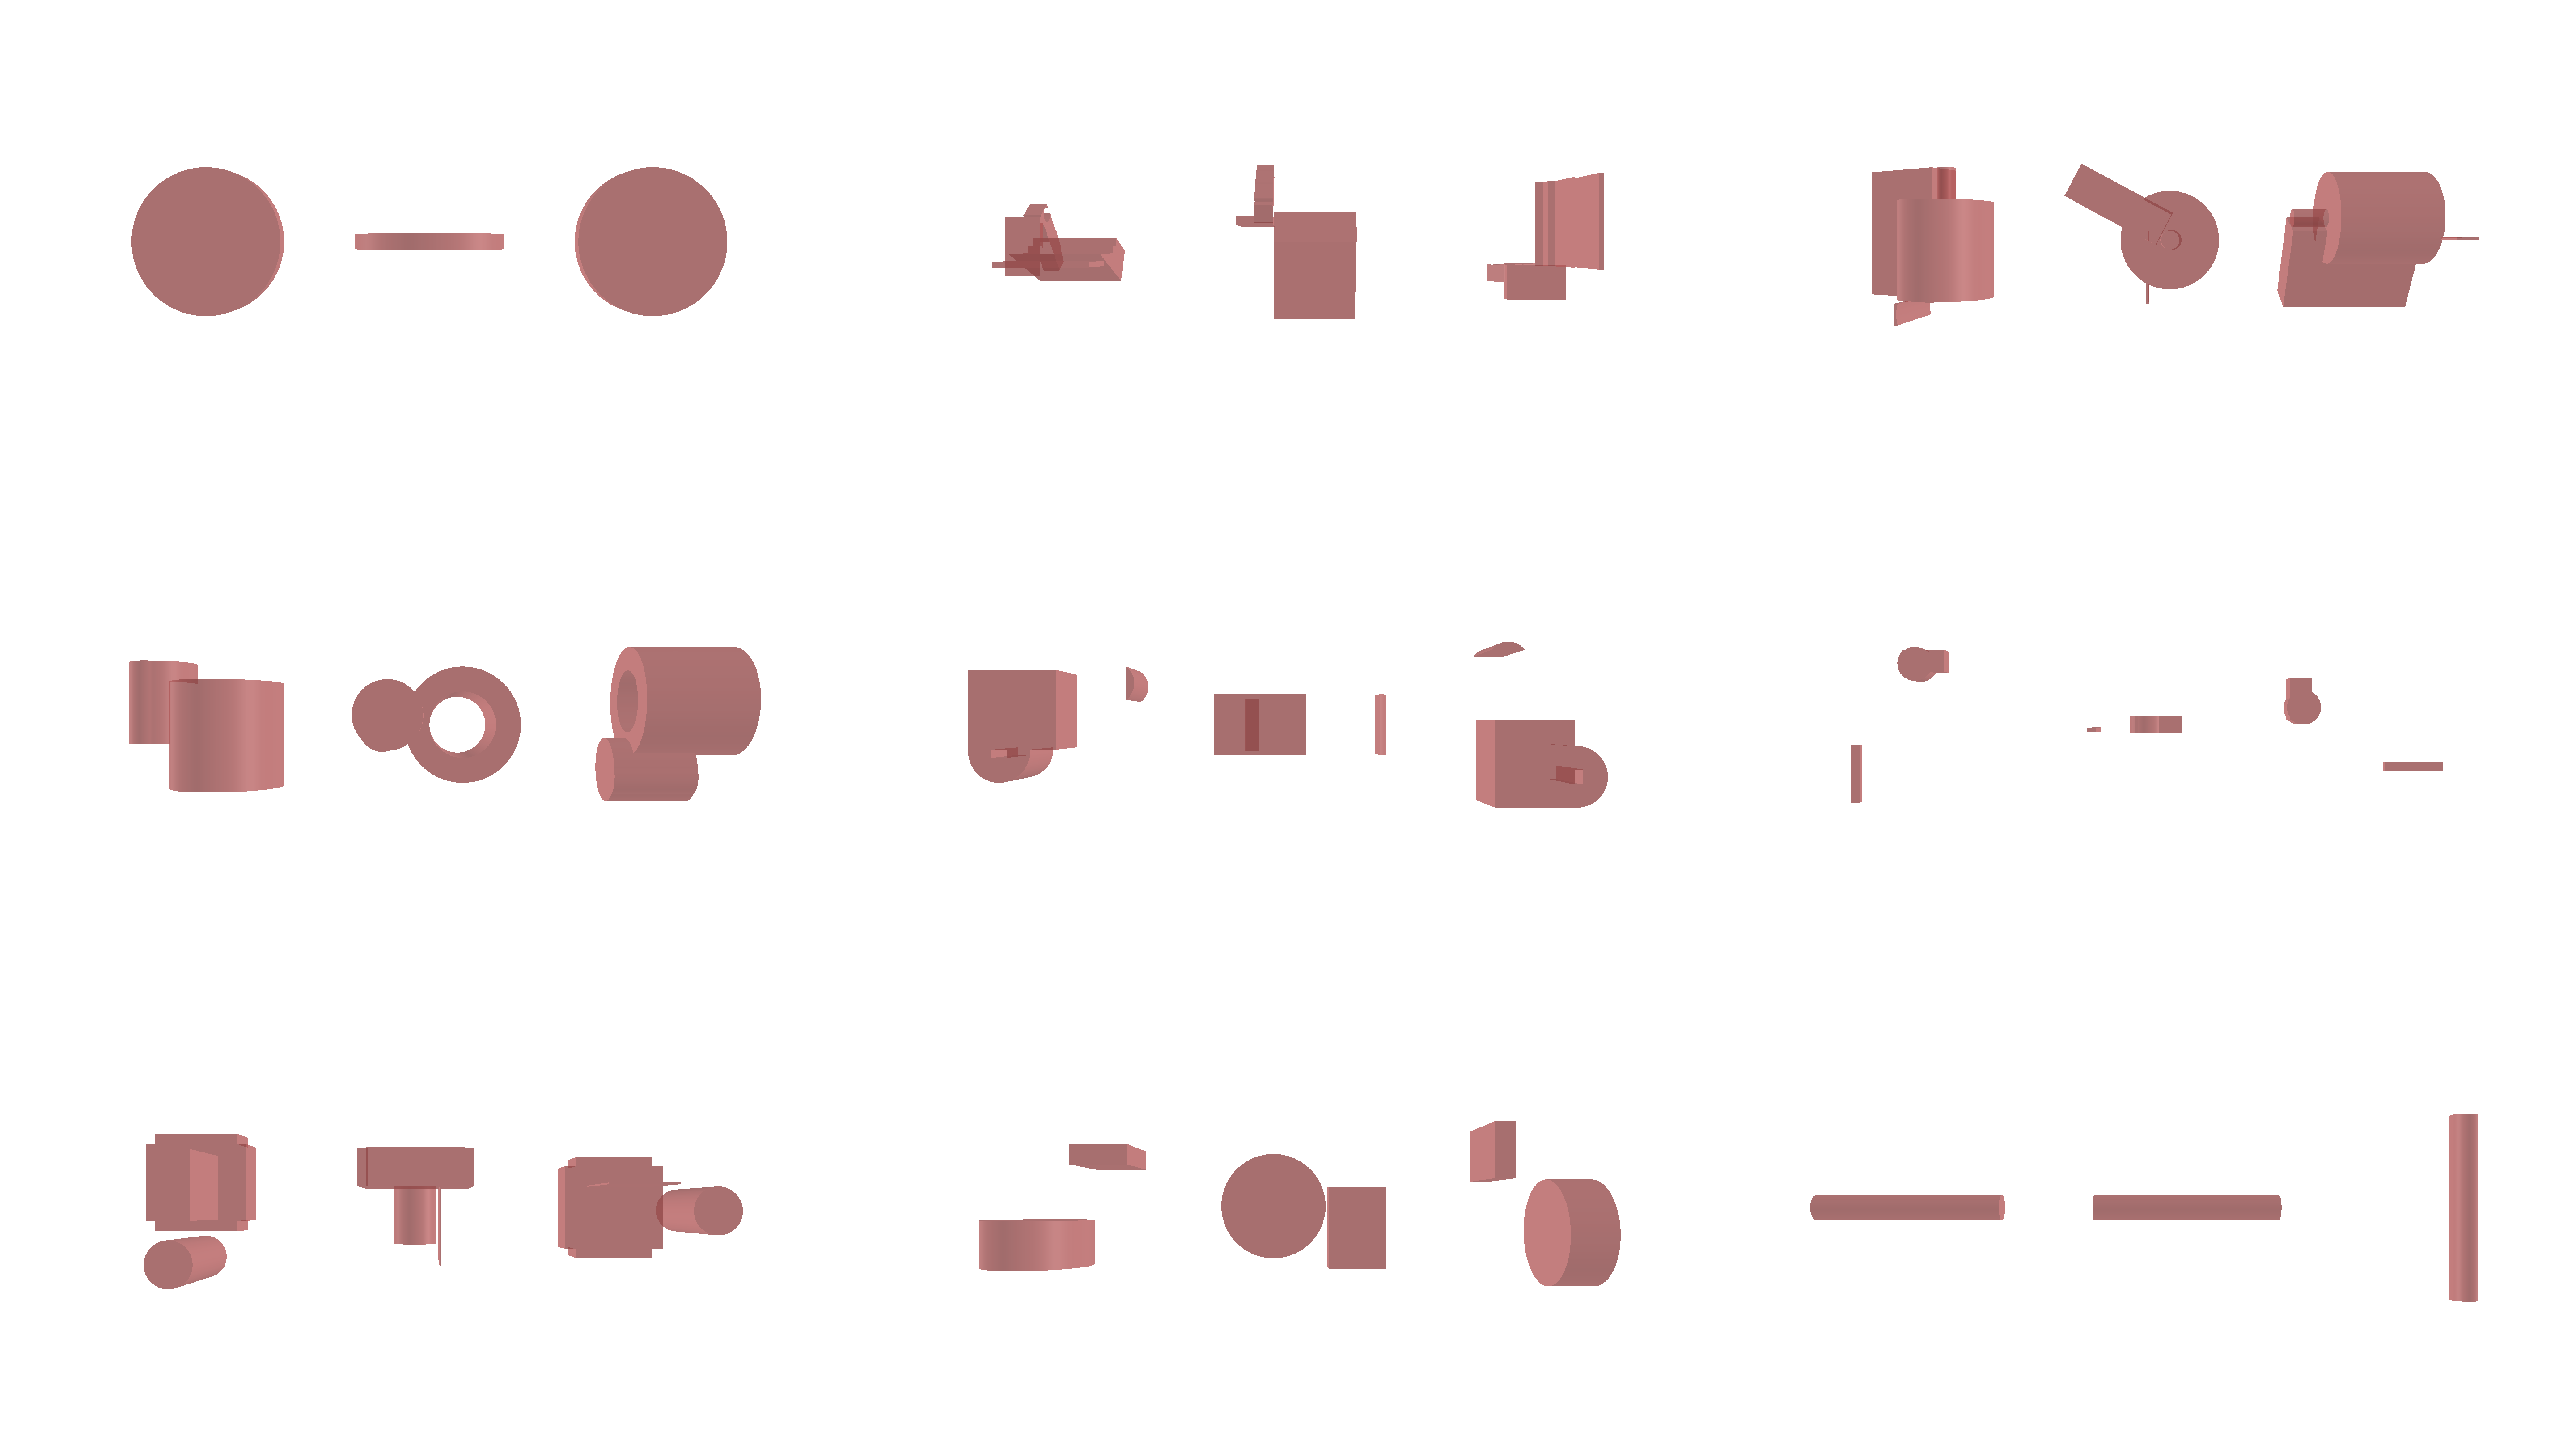
\includegraphics[width=\textwidth]{cadrecode_set.png}
    \caption{CAD-Recode}

    \vspace{1em}

    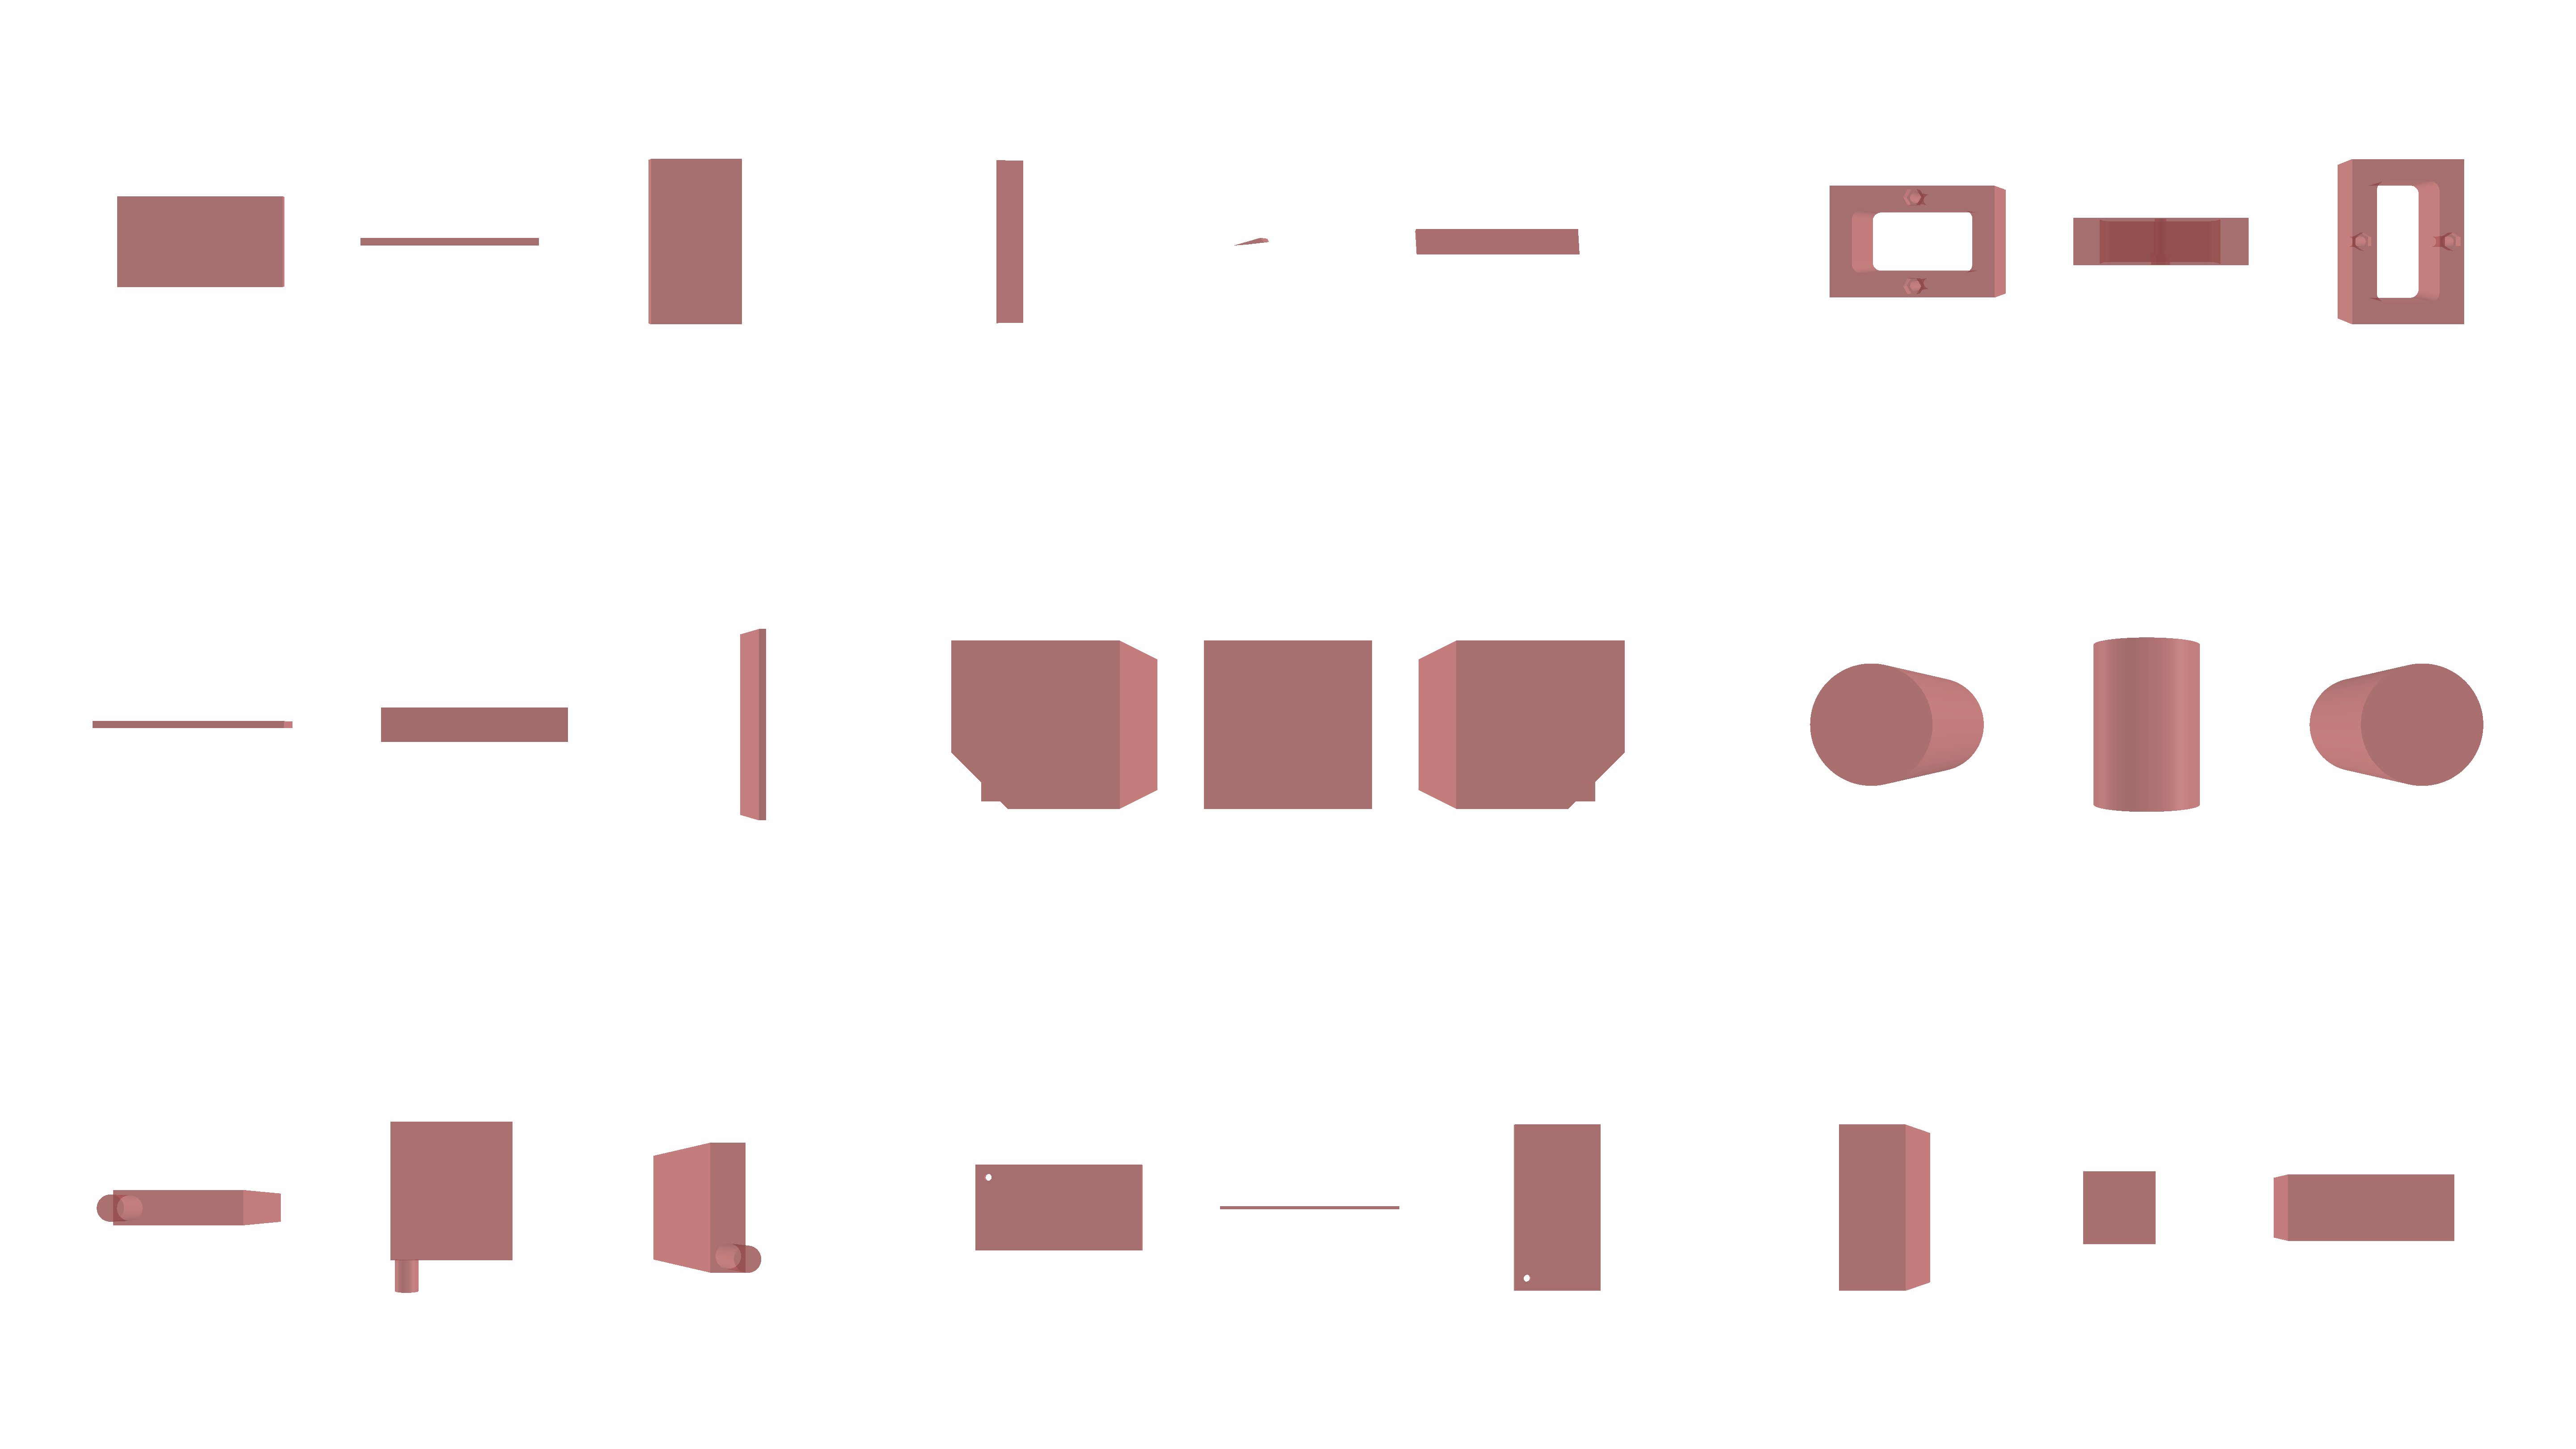
\includegraphics[width=\textwidth]{deepcad_set.png}
    \caption{DeepCAD}

    \caption{Примеры данных из валидационных наборов CAD-Recode и DeepCAD}
    \label{fig:datasets1}
\end{figure}

\newpage

\begin{figure}[h!]
    \centering
    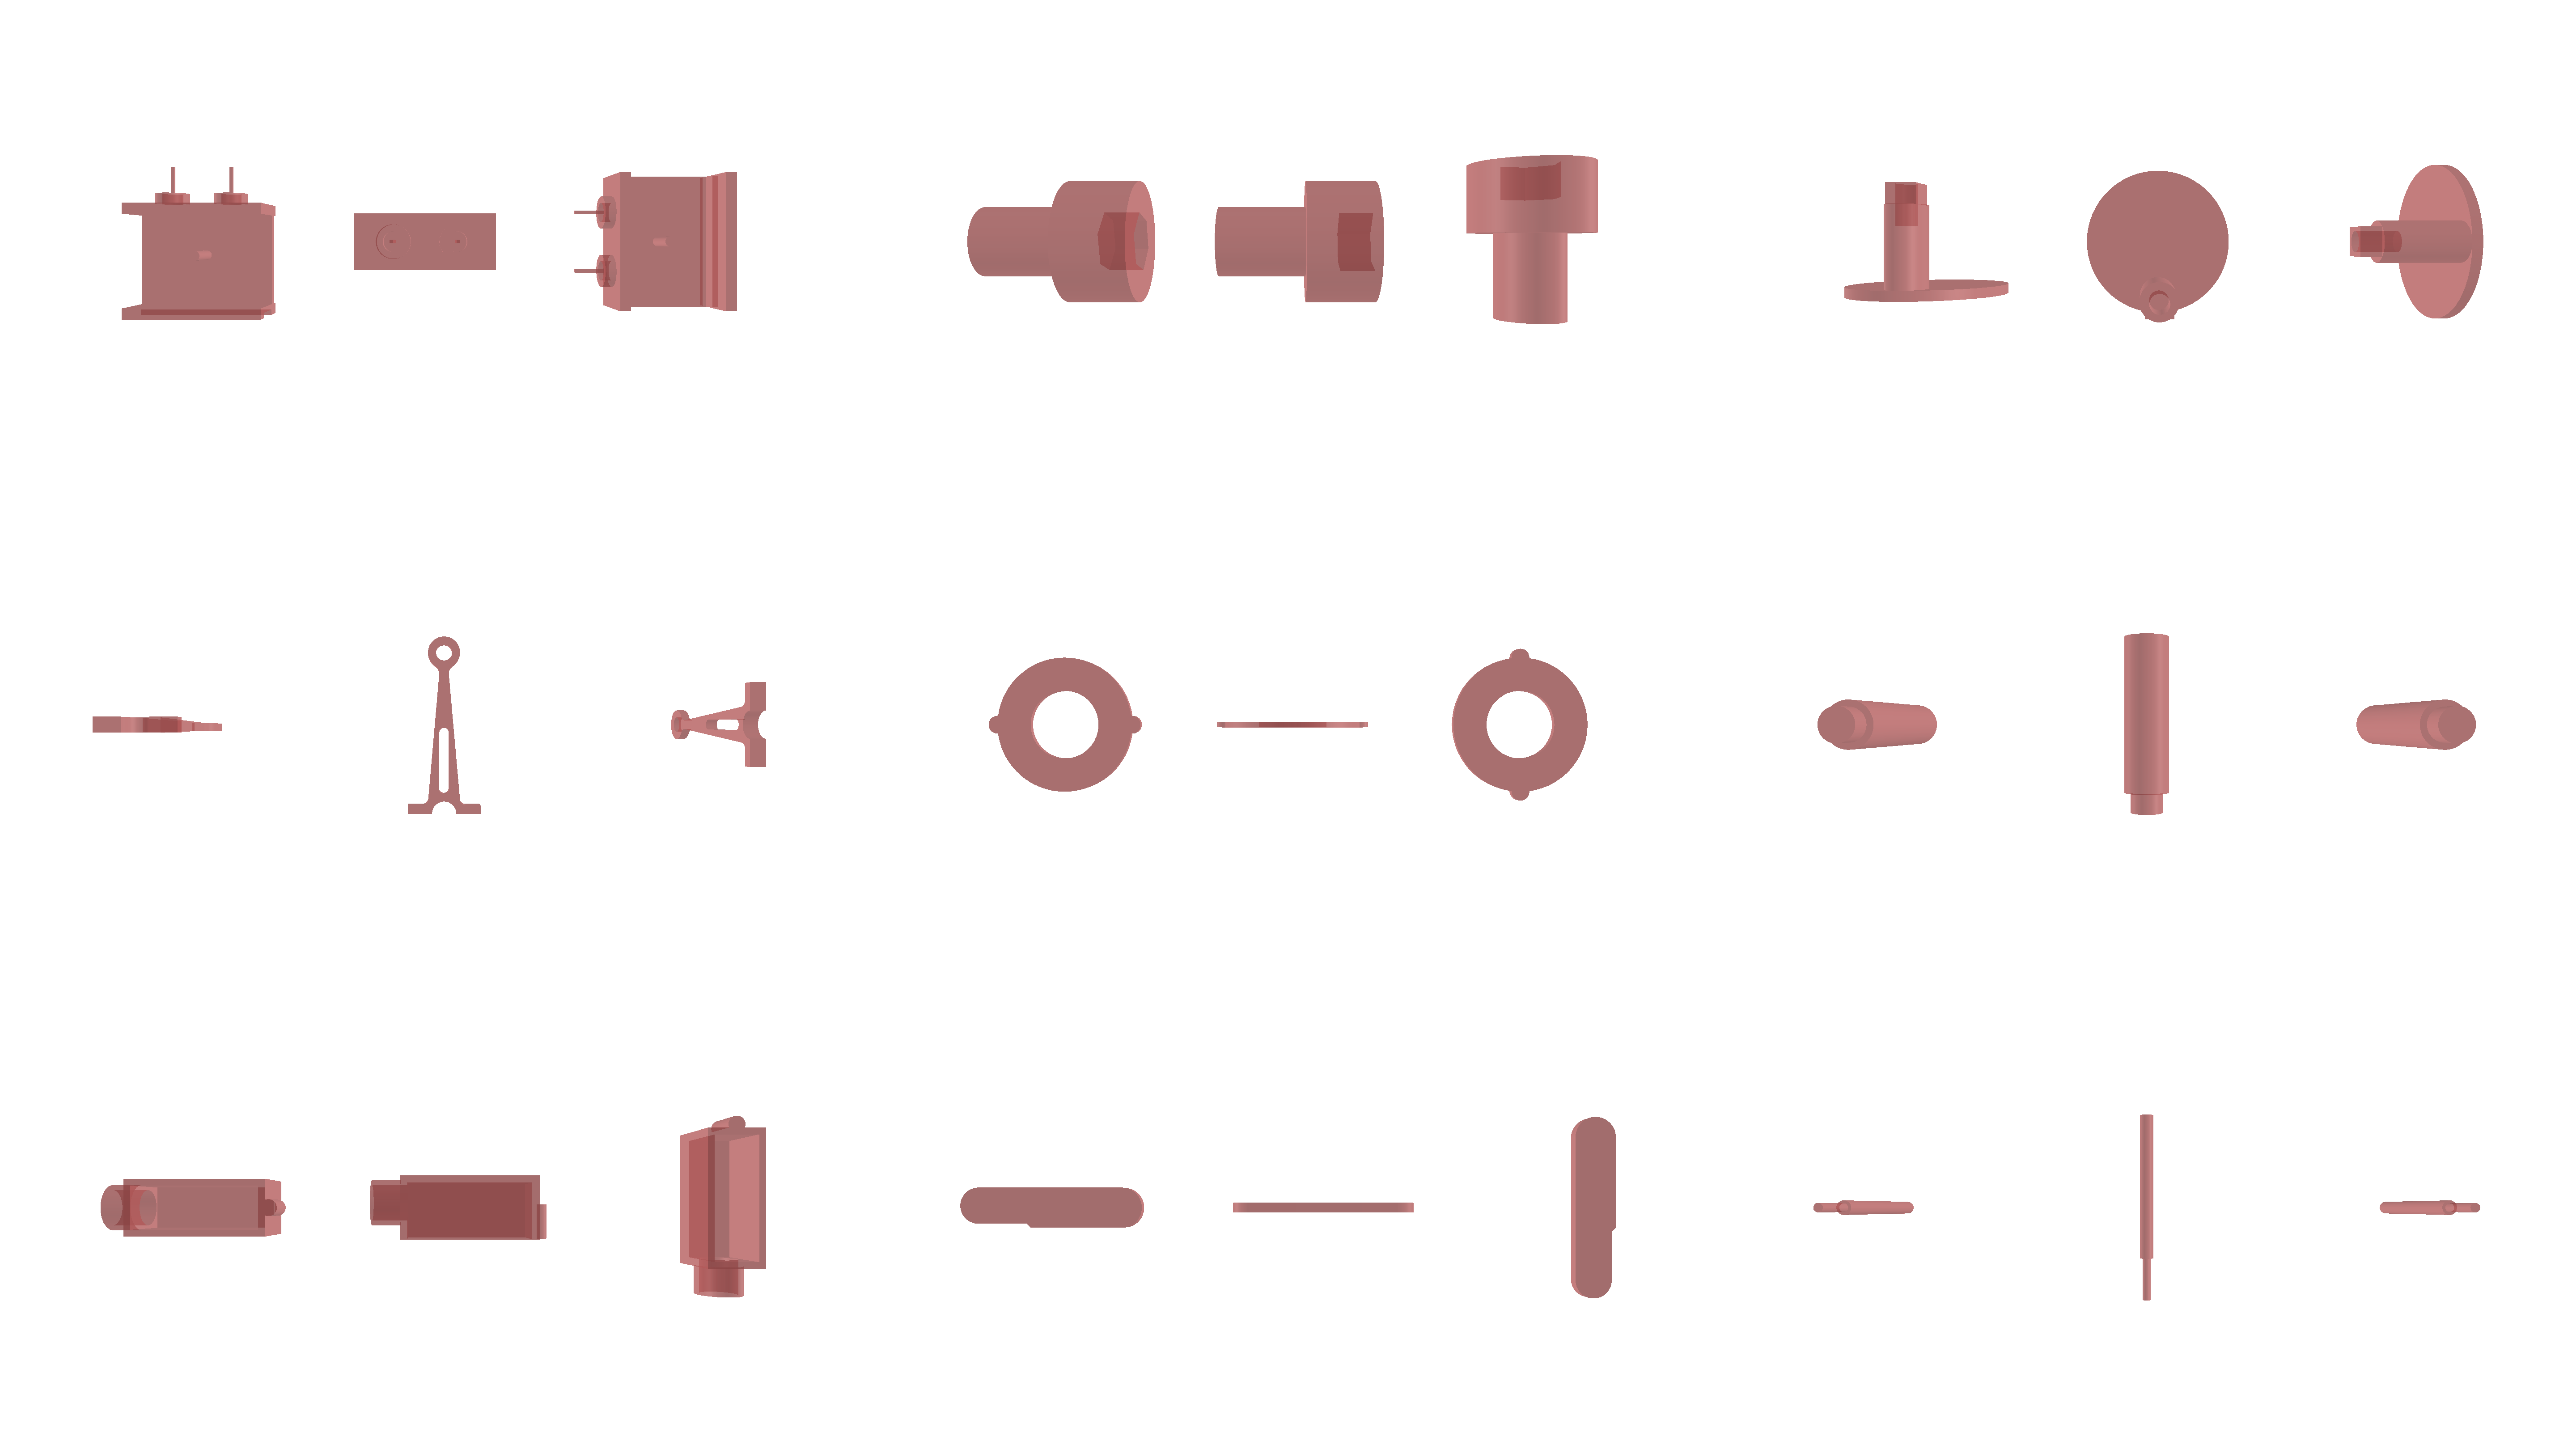
\includegraphics[width=\textwidth]{fusion360_set.png}
    \caption{Fusion360}

    \vspace{1em}

    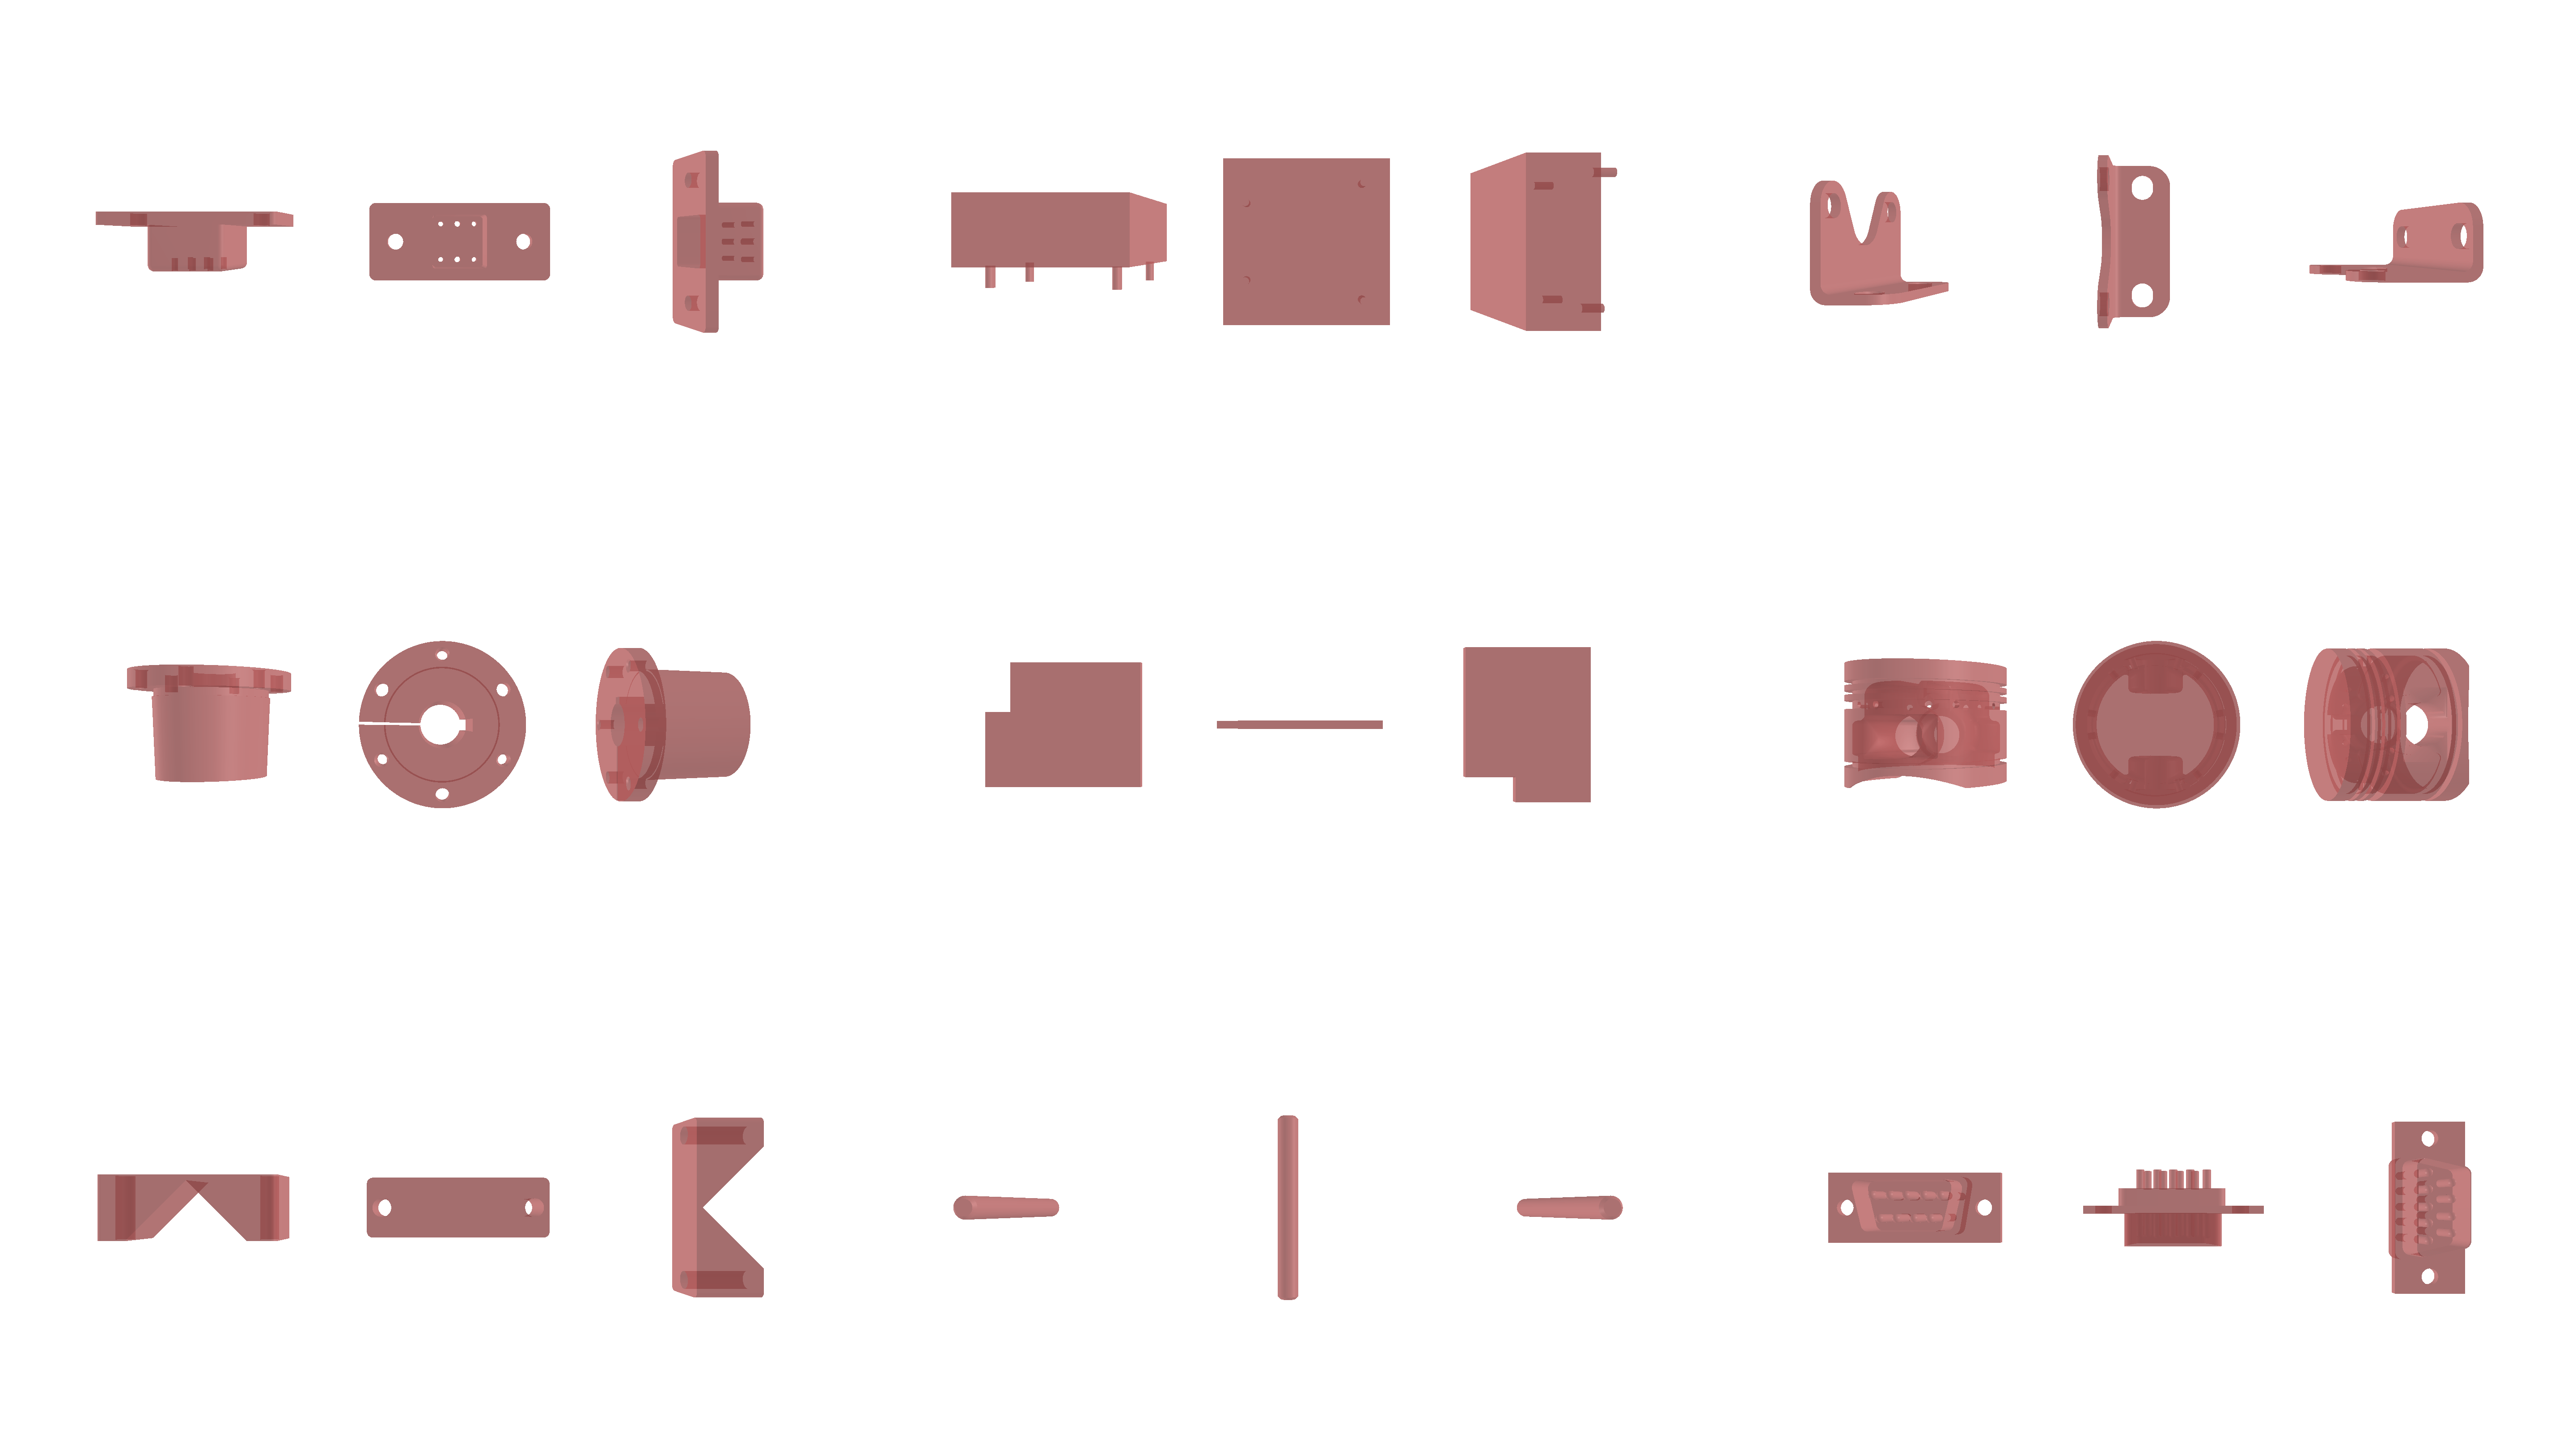
\includegraphics[width=\textwidth]{cc3d_set.png}
    \caption{CC3D}

    \caption{Примеры данных из валидационных наборов Fusion360 и CC3D}
    \label{fig:datasets2}
\end{figure}

\newpage

\subsection{Результаты и анализ.}

Я проведу анализ каждой эпохи на вышеописанных датасетах, это позволит нам понять тренд обучения и проанализировать закономерности.

Сводные таблицы с метриками оказываются очень громоздкими и малоинформативными, поэтому анализ будет произведен на графиках.

\begin{figure}[h!]
    \centering
    \begin{subfigure}{0.45\linewidth}
        \centering
        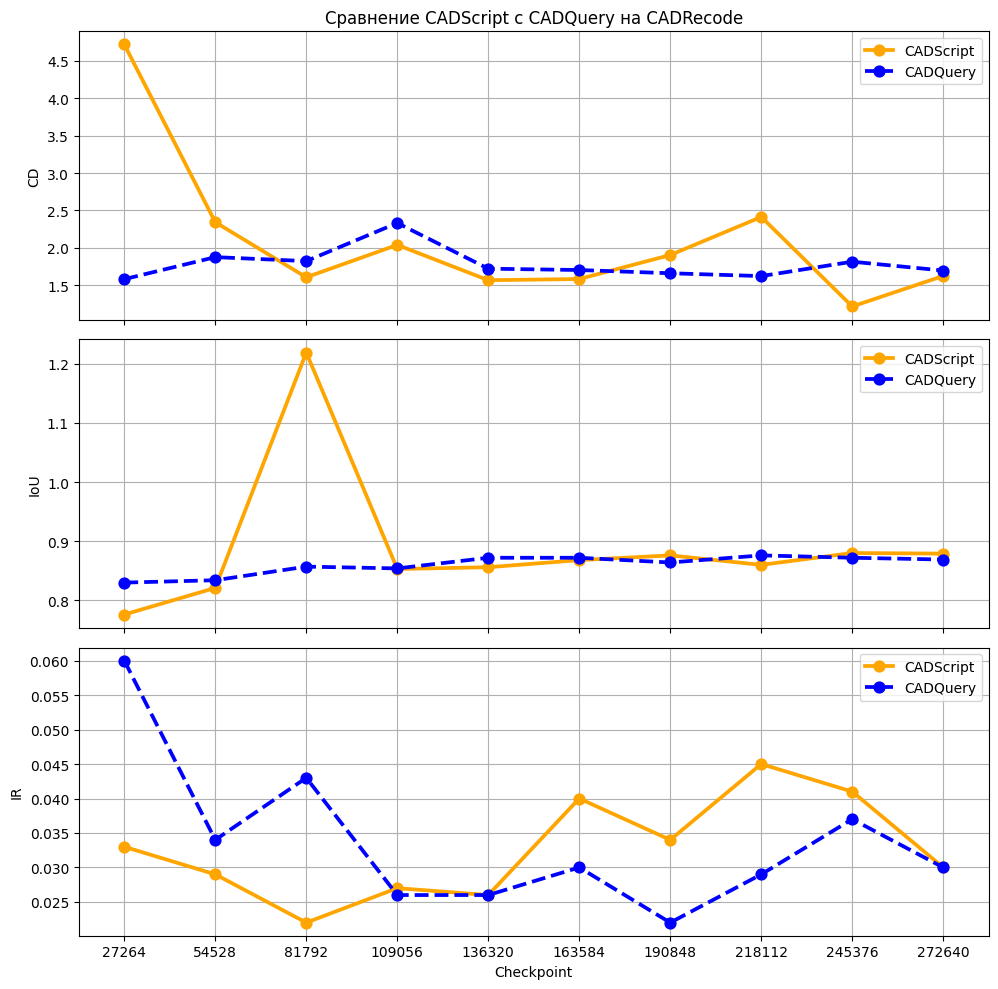
\includegraphics[width=\linewidth]{formats/formats_cadrecode.png}
        \caption{CAD-Recode}
    \end{subfigure}
    \hfill
    \begin{subfigure}{0.45\linewidth}
        \centering
        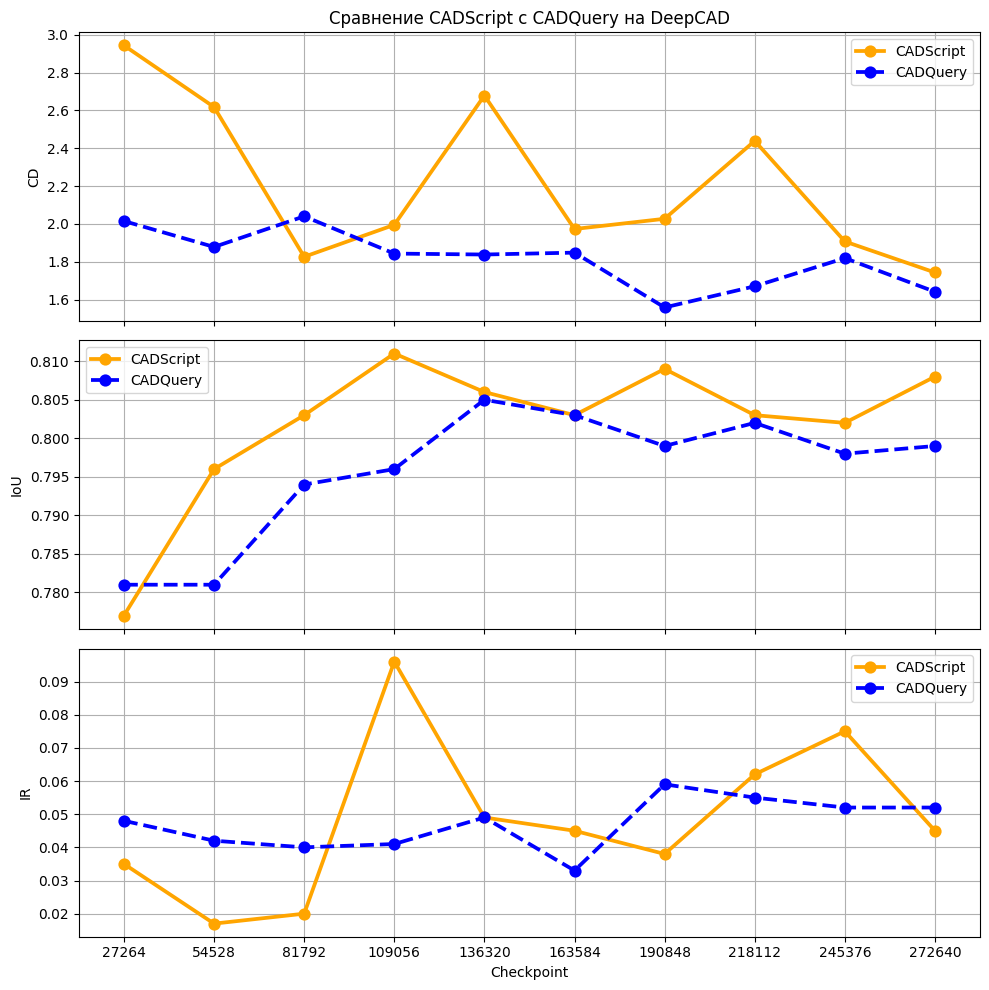
\includegraphics[width=\linewidth]{formats/formats_deepcad.png}
        \caption{DeepCAD}
    \end{subfigure}

    \vspace{1em}

    \begin{subfigure}{0.45\linewidth}
        \centering
        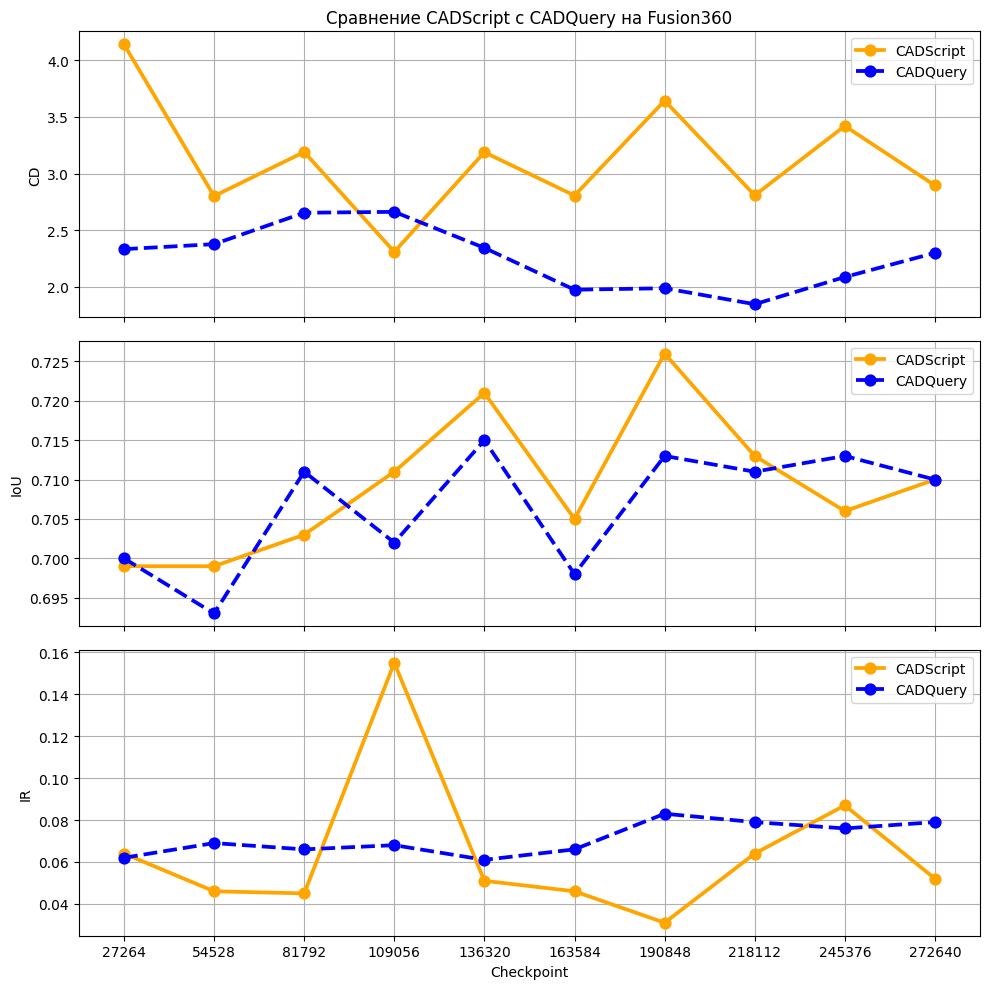
\includegraphics[width=\linewidth]{formats/formats_fusion360.png}
        \caption{Fusion360}
    \end{subfigure}
    \hfill
    \begin{subfigure}{0.45\linewidth}
        \centering
        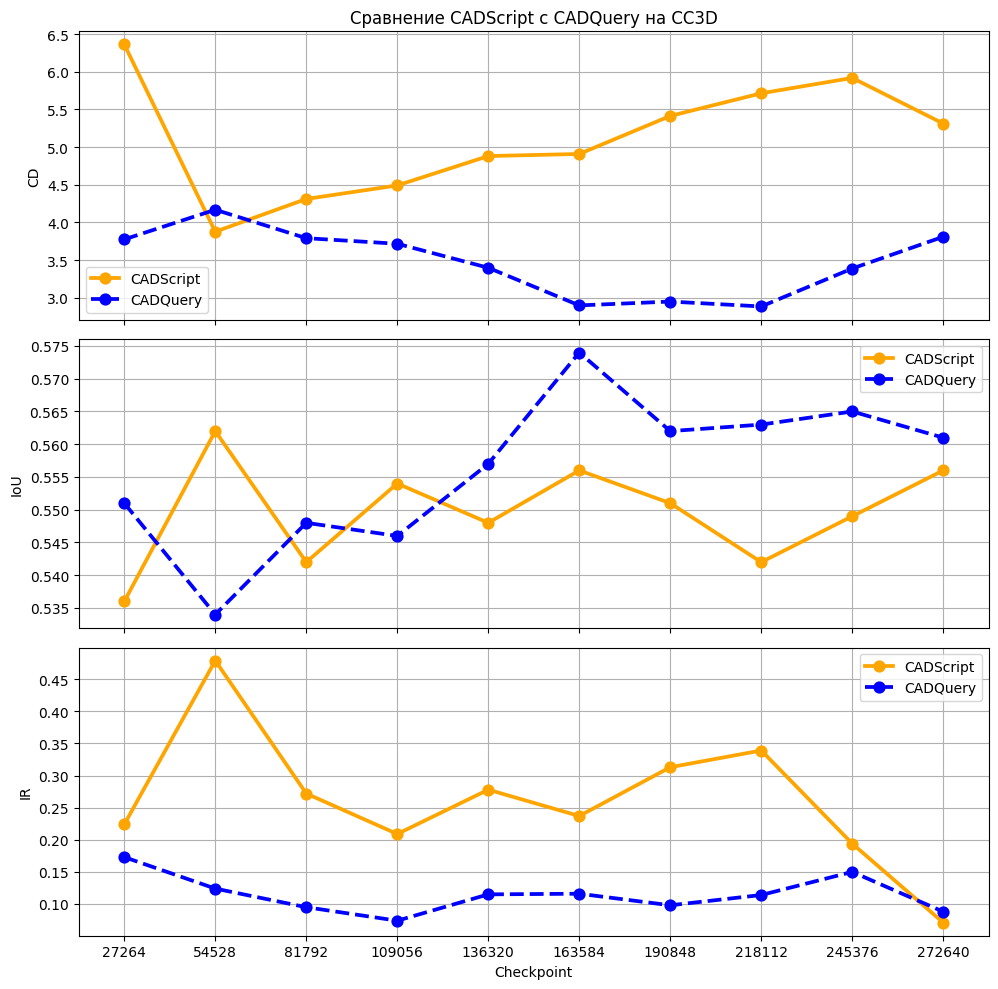
\includegraphics[width=\linewidth]{formats/formats_cc3d.png}
        \caption{CC3D}
    \end{subfigure}

    \caption{Результаты экспериментов на CAD-Recode, DeepCAD, Fusion360 и CC3D.
        Верхний график относится к метрике Chamfer Distance (CD) и чем меньше, тем лучше. Второй график Intersection over Union (IoU) — чем больше, тем лучше.
        Последний относится к Invalid Rate (IR) — чем меньше, тем лучше. CD и IoU подсчитаны только на валидных генерациях.}
    \label{fig:exp1}
\end{figure}

Из графика валидации на CADRecode мы можем сделать вывод, что оба формата успешно выучивают train-данные и на синтетических данных дают по сути одинаковые результаты, разница между которыми крайне мала.
На остальных графиках виден чёткий тренд: CADScript даёт всегда больше Chamfer Distance, чем CADQuery на реальных датасетах DeepCAD, Fusion360 и CC3D.
По метрике Intersection over Union сделать чёткого вывода нельзя: разница на Fusion360 и DeepCAD настолько мала, что больше похожа на дисперсию эксперимента, нежели на тренд, хотя на DeepCAD CADScript показал лучшие результаты.
Однако на самом сложном датасете CC3D CADScript явно работает хуже.

По Invalid Rate также ничего конкретного нельзя утверждать, кроме как на датасете CC3D.

На самом деле именно CC3D показывает проигрыш CADScript перед CADQuery. Однако CADQuery тоже не показывает хорошие метрики на подобном датасете.
Вероятно, проигрыш CADScript перед CADQuery на топологии такой высокой сложности заключается в отсутствии у CADScript базовых макросов для создания бокса или цилиндра, которые есть у CADQuery.
И в то время, когда CADQuery приближает сложную топологию простыми примитивами, CADScript пытается сделать сложный loop. Также различия могут быть вызваны претрейном Qwen на CADQuery, хотя вероятность этого невысока.

Однако если мы даже понимаем, что CADSсript проигрывает CADQuery, мы не можем сказать конкретно, что именно он хуже делает.
Так мы плавно переходим к проблеме, что отсутствуют метрики или валидационные сеты, которые бы оценивали способность модели к каким-то конкретным операциям.

\subsection{Валидационный сет SketchGraph}

В статье \texttt{Computer--Aided Design as Language}~\cite{ganin21_cadlanguage} авторы описывают модель для генерации CAD-эскизов. Архитектура их решения не представляет интереса в рамках данного изложения, однако собранные ими данные оказываются практически полезны.
Для формирования датасета исследователи использовали репозиторий документов, находящихся в открытом доступе на платформе Onshape (Onshape Developers). Результирующий набор данных представлен в виде последовательностей токенов, описывающих геометрические примитивы и отношения между ними (constraints). Это ещё один формат представления скетчей, дополнительно к формату profile-loop.

Конструкции constraints позволяют описывать сложные эскизы значительно меньшим количеством символов. На рисунке~\ref{fig:constraint} приведены примеры MirrorConstraint (зеркалирование), TangentConstraint (касательная), OrthogonalConstraint (перпендикуляр) и CoincidentConstraint (совпадение). Благодаря им, даже без явного указания координат, можно реализовать столь сложную фигуру, как сердце.

\begin{figure}[h!]
    \centering
    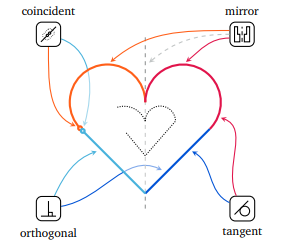
\includegraphics[width=0.5\textwidth]{constraint.png}
    \caption{Примеры constraints}
    \label{fig:constraint}
\end{figure}

Однако не все скетчи оказываются валидными для применения операции Extrude. На рисунке~\ref{fig:sketchgraph} видно, что в вариантах \ref{fig:sg1} и~\ref{fig:sg2} нельзя однозначно определить, что именно является вырезом из внешнего контура.

\begin{figure}[h!]
    \centering
    \begin{subfigure}[b]{0.3\textwidth}
        \centering
        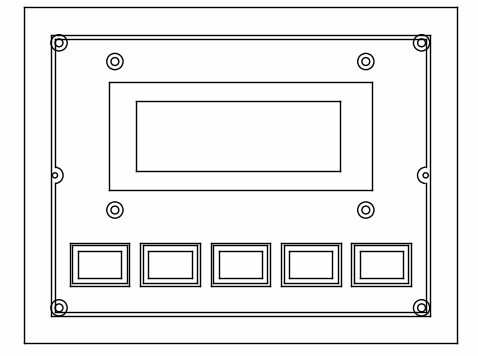
\includegraphics[width=\textwidth]{sg1.png}
        \caption{}
        \label{fig:sg1}
    \end{subfigure}
    \hfill
    \begin{subfigure}[b]{0.3\textwidth}
        \centering
        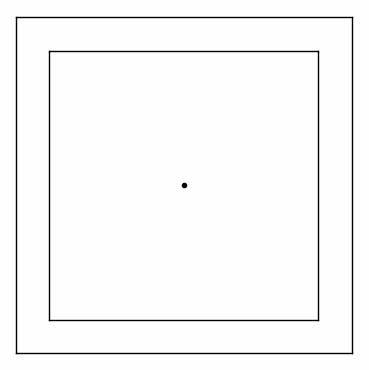
\includegraphics[width=\textwidth]{sg2.png}
        \caption{}
        \label{fig:sg2}
    \end{subfigure}
    \hfill
    \begin{subfigure}[b]{0.3\textwidth}
        \centering
        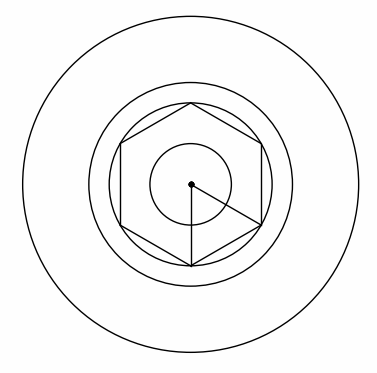
\includegraphics[width=\textwidth]{sg3.png}
        \caption{}
        \label{fig:sg3}
    \end{subfigure}
    \caption{Примеры скетчей из SketchGraph}
    \label{fig:sketchgraph}
\end{figure}

Чтобы решить эту проблему, можно взять все возможные замкнутые контуры (loop) в SketchGraph и выделить их подмножества, которые образуют валидный profile. Затем остаётся лишь перевести constraints в парадигму loop-profile, и мы получим валидные скетчи, которые можно сохранить в формате CADAxt.

Благодаря интеграции CADAxt с синтетическим генератором возможно выполнить экструдирование полученных эскизов. Таким образом формируется набор 3D-моделей, которые получены при помощи рисования скетчей различной сложности с последующей операцией Extrude.

Эти 3D-модели разделяют на три класса по уровню сложности:
\begin{enumerate}
    \item Простые: количество граней в интервале $(5, 15]$.
    \item Средние: количество граней в интервале $(15, 30]$.
    \item Сложные: количество граней в интервале $(30, 50]$.
\end{enumerate}

В итоге получается набор 3D-моделей, созданных одной операцией Extrude и разбитых на три класса. На рисунке~\ref{fig:sketchgraph_set} показан пример такого набора: слева направо приведено по 9 представителей каждого класса от сложных к простым.

\begin{figure}[h!]
    \centering
    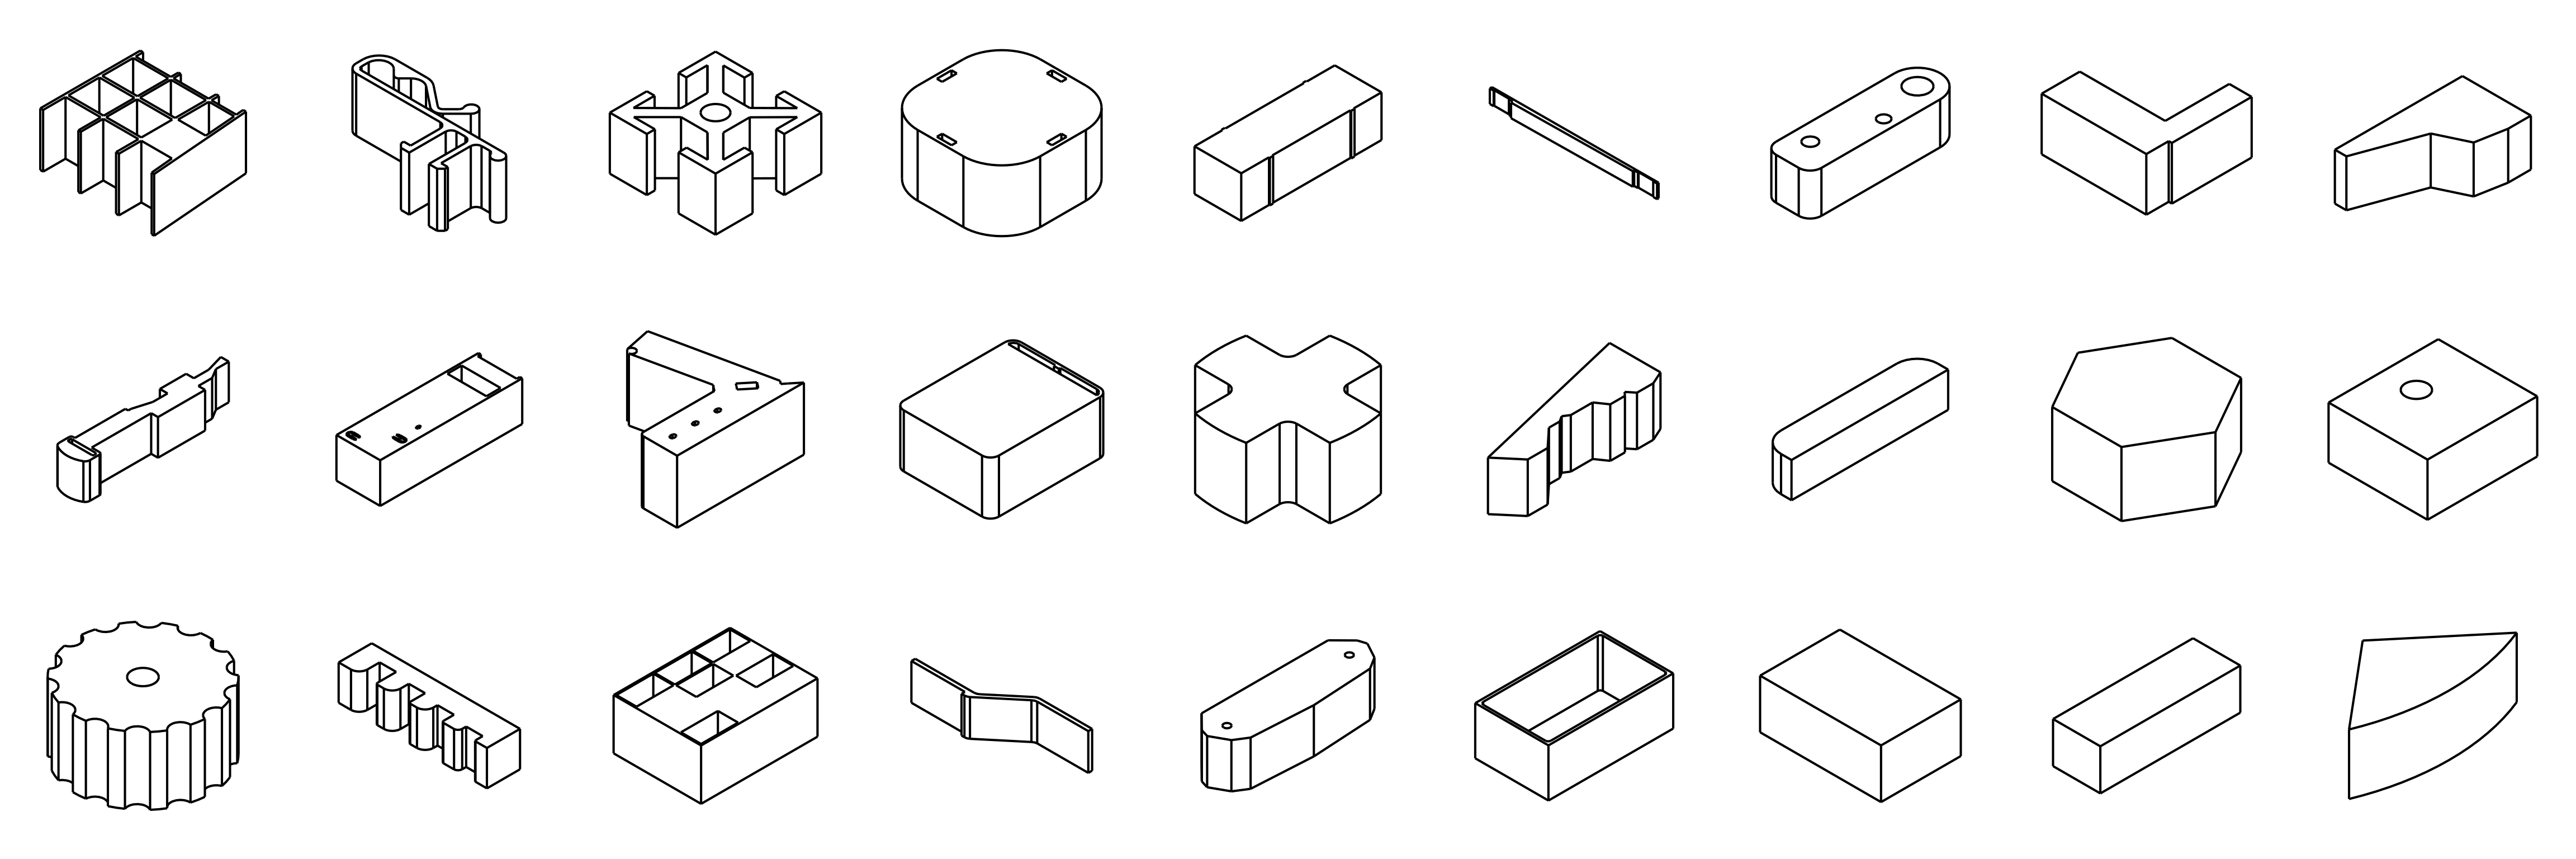
\includegraphics[width=\textwidth]{sketchgraph_set.png}
    \caption{Валидационный сет SketchGraph: примеры 3D-моделей, распределённых по сложности (сложные, средние, простые).}
    \label{fig:sketchgraph_set}
\end{figure}

Основная задача данного валидационного набора:
\begin{enumerate}
    \item Проверить способность модели воспроизводить представленные 3D-модели за одну операцию Extrude.
    \item Оценить, как модель справляется с топологиями разной сложности.
\end{enumerate}

\paragraph{Сравнение CADScript и CADQuery на SketchGraph.}

Теперь можно проверить, насколько эффективно наши два представления (CADScript и CADQuery) способны рисовать скетчи.

\begin{figure}[h!]
    \centering
    \begin{subfigure}{0.45\linewidth}
        \centering
        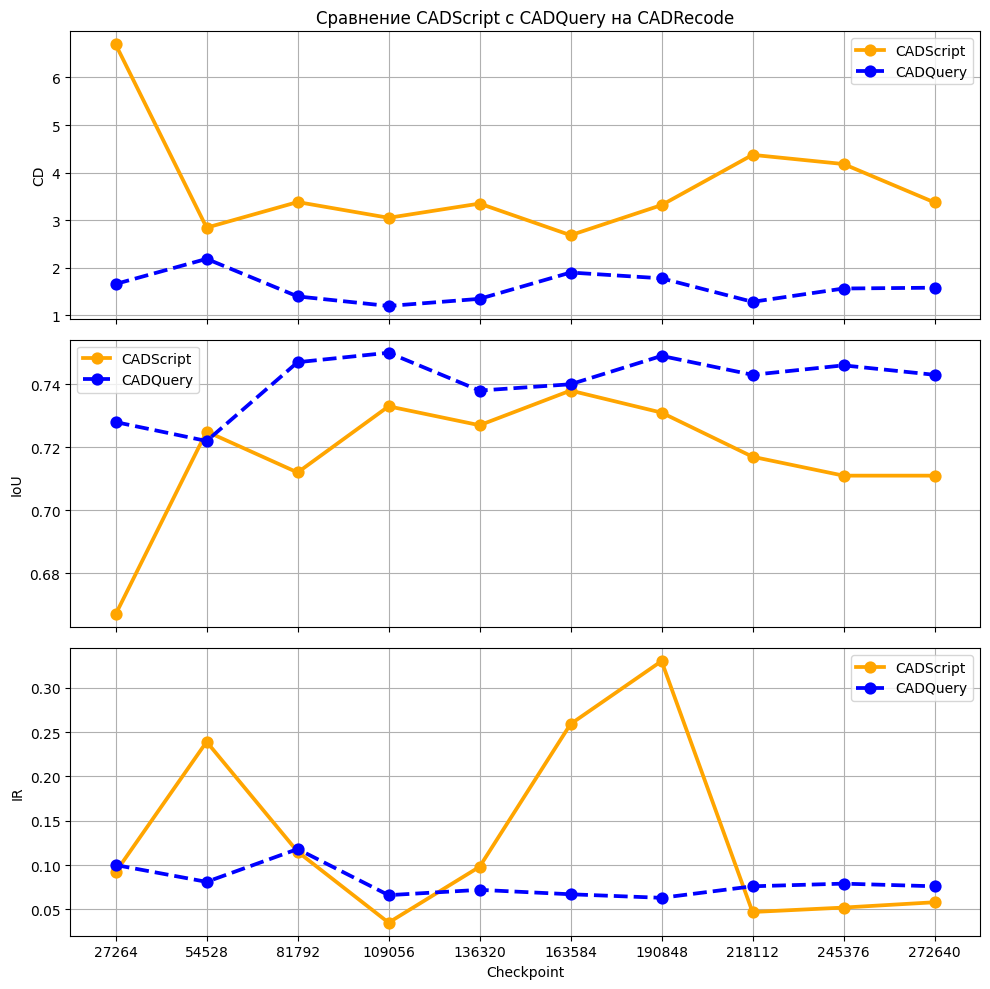
\includegraphics[width=\linewidth]{formats/formats_sketchgraph.png}
        \caption{На всём наборе данных}
    \end{subfigure}
    \hfill
    \begin{subfigure}{0.45\linewidth}
        \centering
        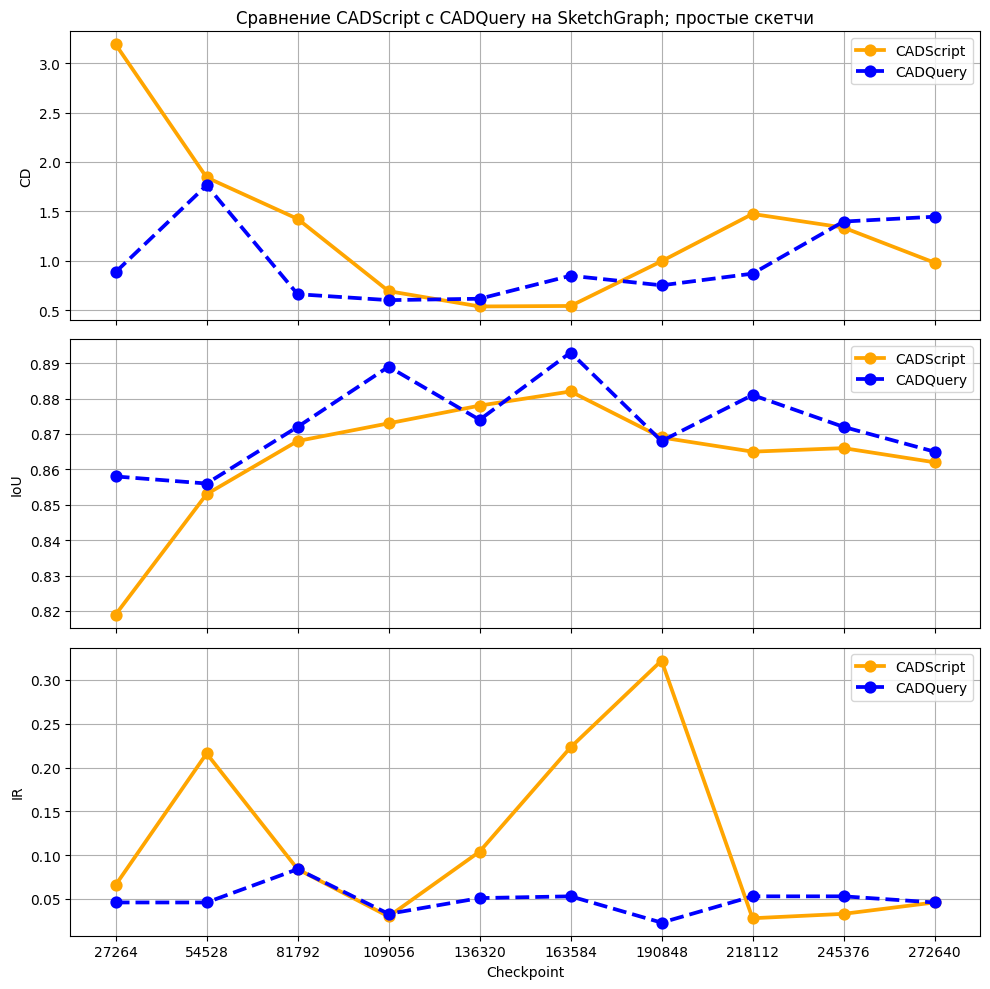
\includegraphics[width=\linewidth]{formats/formats_sketchgraph_easy.png}
        \caption{Простые скетчи}
    \end{subfigure}

    \vspace{1em}

    \begin{subfigure}{0.45\linewidth}
        \centering
        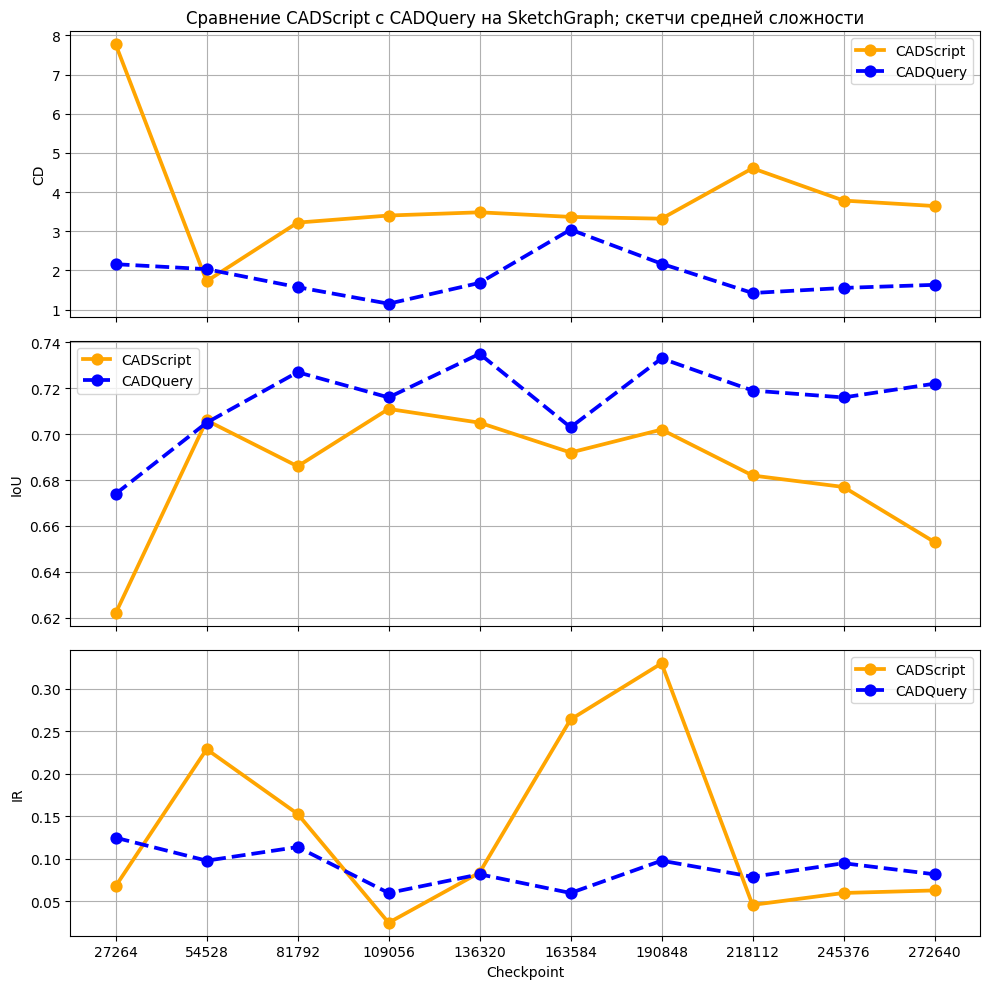
\includegraphics[width=\linewidth]{formats/formats_sketchgraph_medium.png}
        \caption{Скетчи средней сложности}
    \end{subfigure}
    \hfill
    \begin{subfigure}{0.45\linewidth}
        \centering
        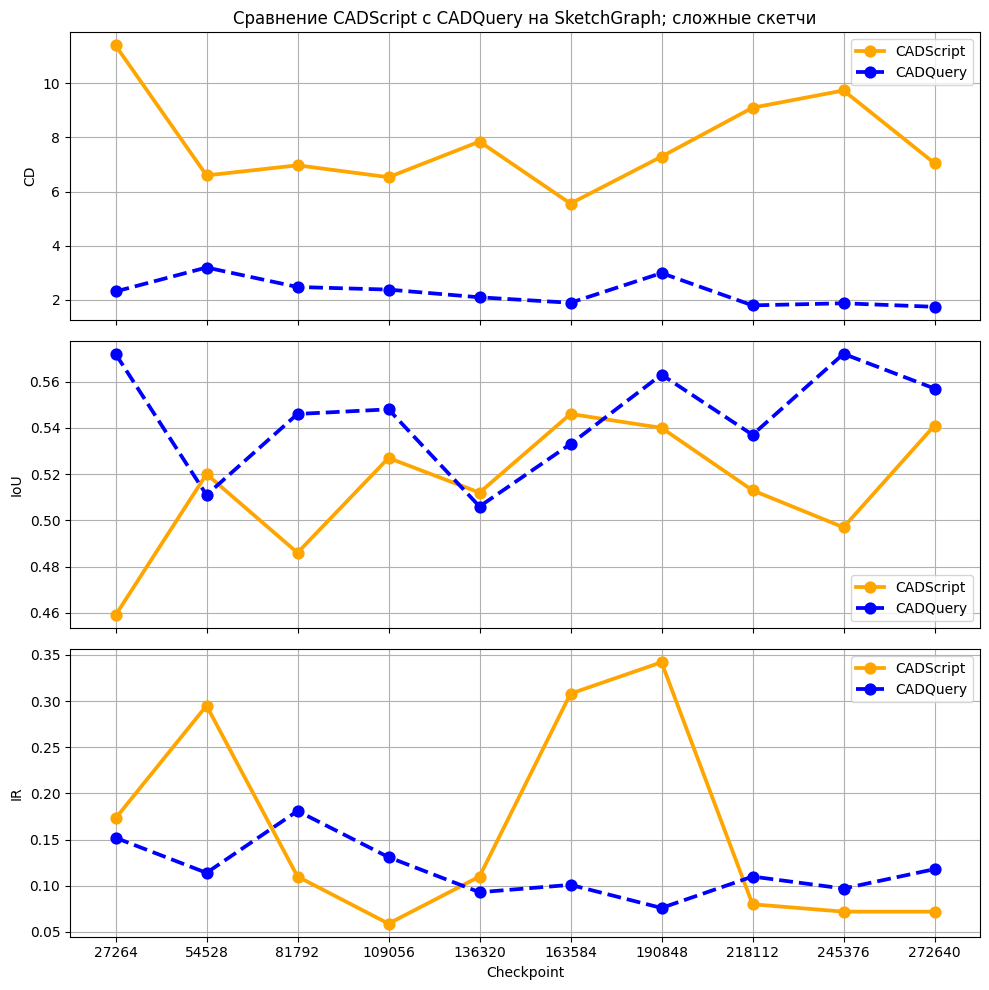
\includegraphics[width=\linewidth]{formats/formats_sketchgraph_hard.png}
        \caption{Сложные скетчи}
    \end{subfigure}

    \caption{Результаты экспериментов на SketchGraph и на трёх классах по уровню сложности топологии.
        Верхний график иллюстрирует метрику Chamfer Distance (CD), где меньшее значение лучше.
        Второй график --- Intersection over Union (IoU), где большее значение лучше.
        Третий график --- Invalid Rate (IR), где меньшее значение лучше.
        Метрики CD и IoU подсчитаны только на валидных генерациях.}
    \label{fig:exp2}
\end{figure}

Из графиков (рис.~\ref{fig:exp2}) хорошо видно, что на простых скетчах результаты CADScript и CADQuery сопоставимы. Однако на средних и сложных скетчах CADScript уступает CADQuery по метрикам CD и IoU, а показатель Invalid Rate сильно колеблется. Может возникнуть мысль, что CADQuery просто приближает топологию (за счёт большого числа простых команд) и поэтому показывает более высокие результаты, тогда как CADScript действительно старается точно воспроизводить скетчи. Или же CADQuery всегда использует простейшие макросы (cylinder/box) и, благодаря этому, повышает свои показатели.

Чтобы разобраться в этом, введём две дополнительные метрики:
\begin{enumerate}
    \item Extrude Mean (EM) --- среднее количество операций extrude.
    \item Base Extrude Ratio (BER) --- отношение числа простейших макросов (cylinder и
          box) у CADQuery ко всем его командам extrude.
\end{enumerate}

По этим метрикам получены следующие результаты:

\begin{figure}[h!]
    \centering
    \begin{subfigure}{0.45\linewidth}
        \centering
        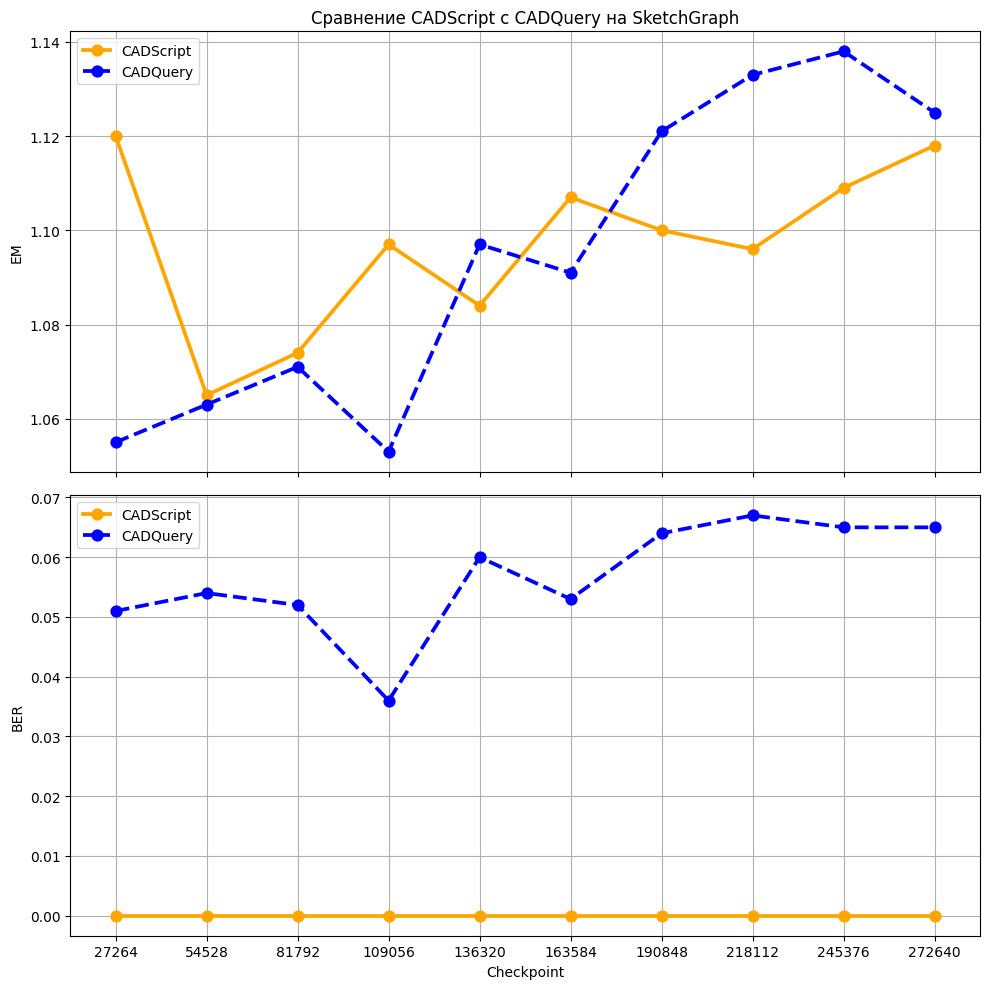
\includegraphics[width=\linewidth]{formats/format_em.png}
        \caption{На всём наборе данных}
    \end{subfigure}
    \hfill
    \begin{subfigure}{0.45\linewidth}
        \centering
        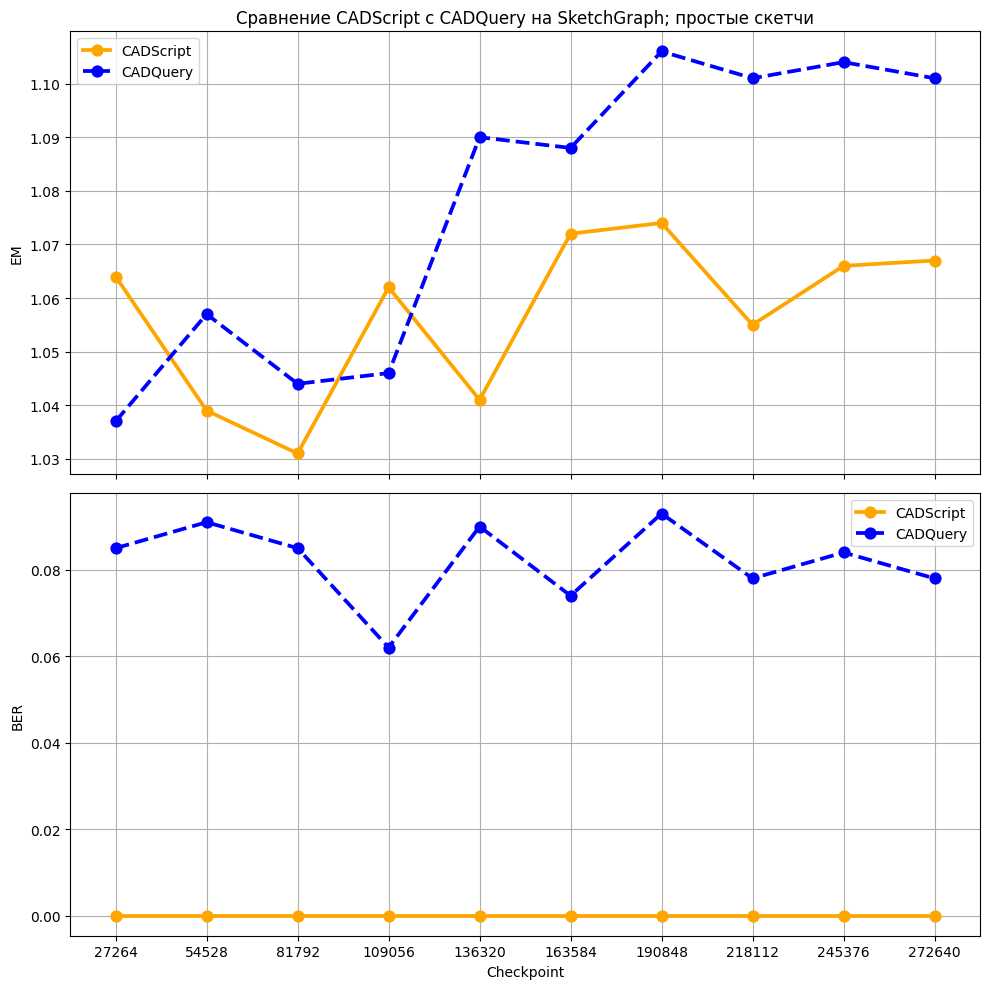
\includegraphics[width=\linewidth]{formats/format_em_e.png}
        \caption{Простые скетчи}
    \end{subfigure}

    \vspace{1em}

    \begin{subfigure}{0.45\linewidth}
        \centering
        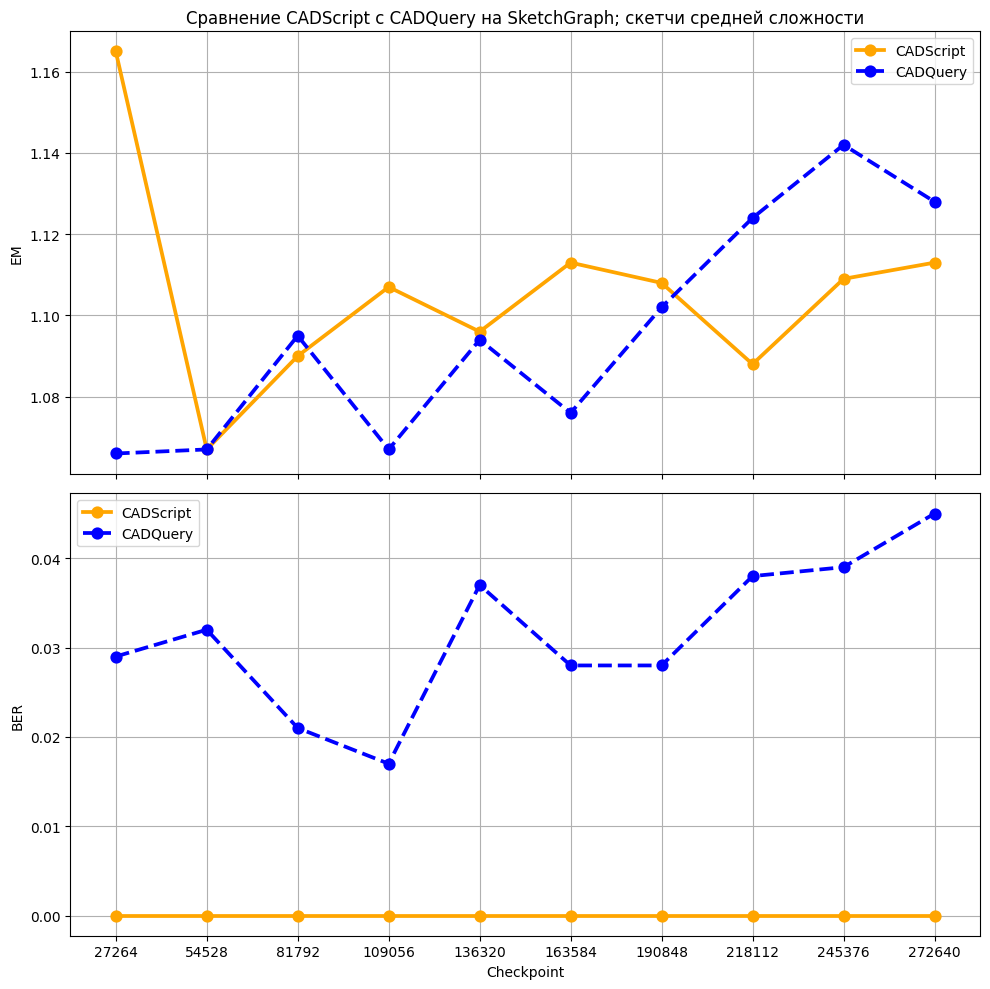
\includegraphics[width=\linewidth]{formats/format_em_m.png}
        \caption{Скетчи средней сложности}
    \end{subfigure}
    \hfill
    \begin{subfigure}{0.45\linewidth}
        \centering
        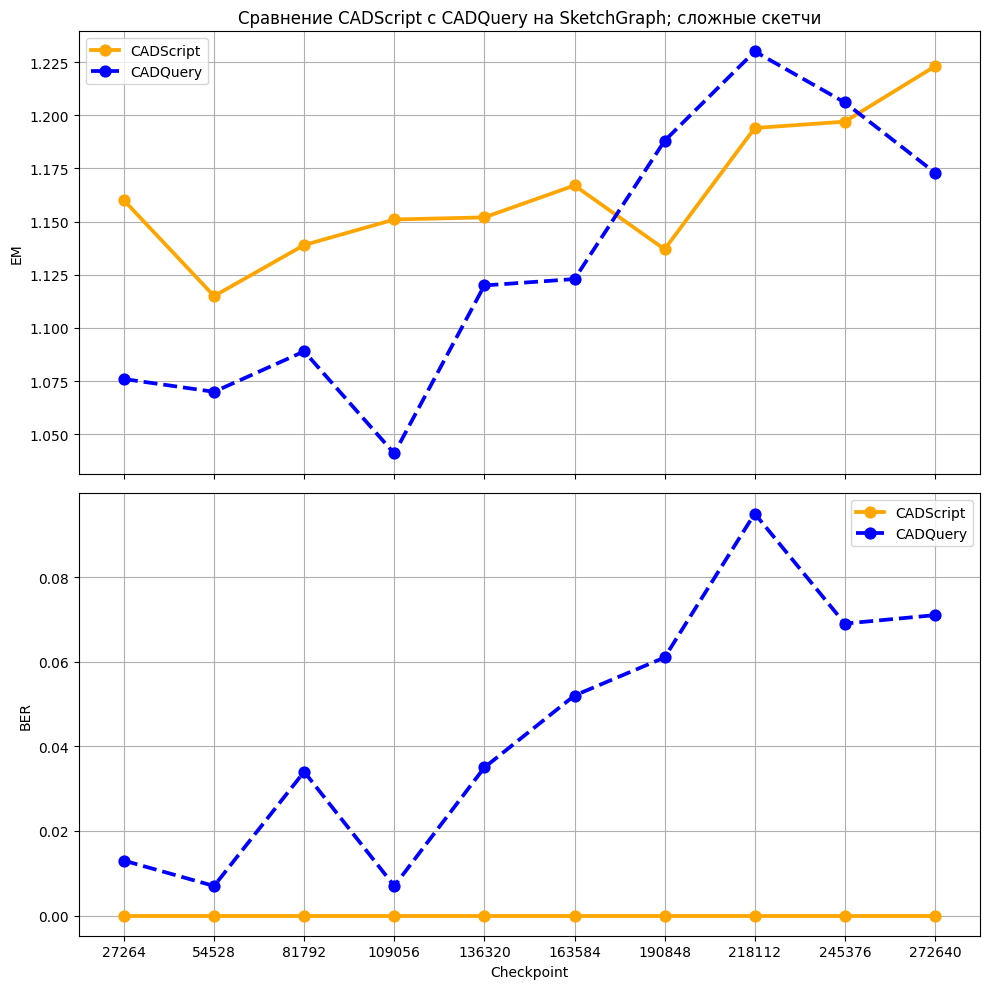
\includegraphics[width=\linewidth]{formats/format_em_h.png}
        \caption{Сложные скетчи}
    \end{subfigure}

    \caption{Результаты по метрикам Extrude Mean (EM) и Base Extrude Ratio (BER) на SketchGraph и на трёх классах по уровню сложности топологии.
        EM (верхний график) показывает среднее число команд extrude (чем меньше, тем лучше).
        BER (нижний график) отражает долю простейших макросов (cylinder или box) у CADQuery; желательно, чтобы она не была слишком большой.}
    \label{fig:exp3}
\end{figure}

Из рис.~\ref{fig:exp3} видно, что CADQuery и CADScript в среднем используют сопоставимое число команд extrude, близкое к единице. При этом доля простейших макросов у CADQuery не превышает 9\,\%,
то есть CADQuery не злоупотребляет такими командами. Следовательно, CADQuery действительно лучше справляется с задачей рисования скетчей, чем CADScript.
Причиной этому может служить то, что в CADScript требуется явное задание описания Loop, в то время как в CADQuery оно происходит неявно.

Таким образом, формат CADQuery предпочтительнее формата CADScript: на реальных данных он даёт меньшие значения метрики CD и лучше справляется с задачей рисования скетчей.

\newpage

\subsection{Тестирование экспериментов на SketchGraph}

Набор данных SketchGraph служит удобным средством для валидации и сравнения новых архитектур. Авторы работы \texttt{CADRille}~\cite{kolodiazhnyi25_cadrille} применили дообучение с подкреплением (RL finetune) к уже обученной модели, основанной на данных DeepCAD и Fusion360. Для этого они использовали метод GRPO, функция потерь которого описывается соответствующим лоссом. Их основной целью было минимизировать показатель Invalid Rate (IR), не снижая метрику Intersection over Union (IoU). Введённая ими функция вознаграждения (reward) предполагала штраф в \(-10\) за несгенерированный семпл и вознаграждение в размере \(+ \mathrm{iou} \times 10\) за успешно сгенерированный.

Хотя такая схема действительно улучшила результаты на датасетах DeepCAD и Fusion360, концептуально она может привести к поведению, при котором модель старается генерировать упрощённую топологию и постепенно «доращивать» её до итога (напоминающее «покадровое» приближение). При таком подходе модель не получает штрафов за IR и постепенно учится повышать IoU. Поэтому важно проверить, что при таком дообучении модель не утрачивает способность корректно рисовать сложные скетчи.

В своих экспериментах я обучал модель CADRecode по схеме RL finetune с использованием GRPO, как в работе авторов \texttt{CADRille}~\cite{kolodiazhnyi25_cadrille}. Обучение длилось 4 дня на 8 GPU H100 на подвыборке из 10\,000 семплов (20 эпох). Итоговые результаты представлены на рисунке~\ref{fig:exp4}.

\newpage
\begin{figure}[h!]
    \centering
    \begin{subfigure}{0.4\linewidth}
        \centering
        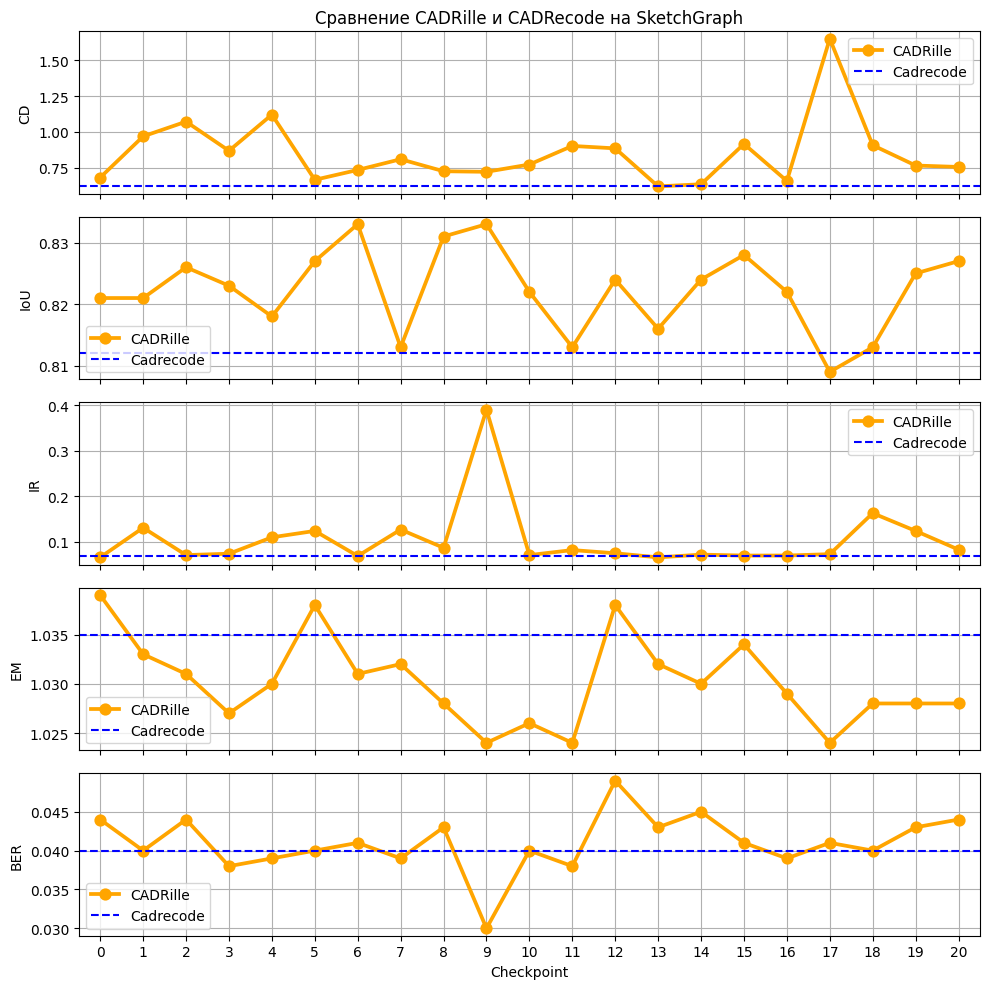
\includegraphics[width=\linewidth]{cadrille_sketchgraph.png}
        \caption{На всём наборе данных}
    \end{subfigure}
    \hfill
    \begin{subfigure}{0.4\linewidth}
        \centering
        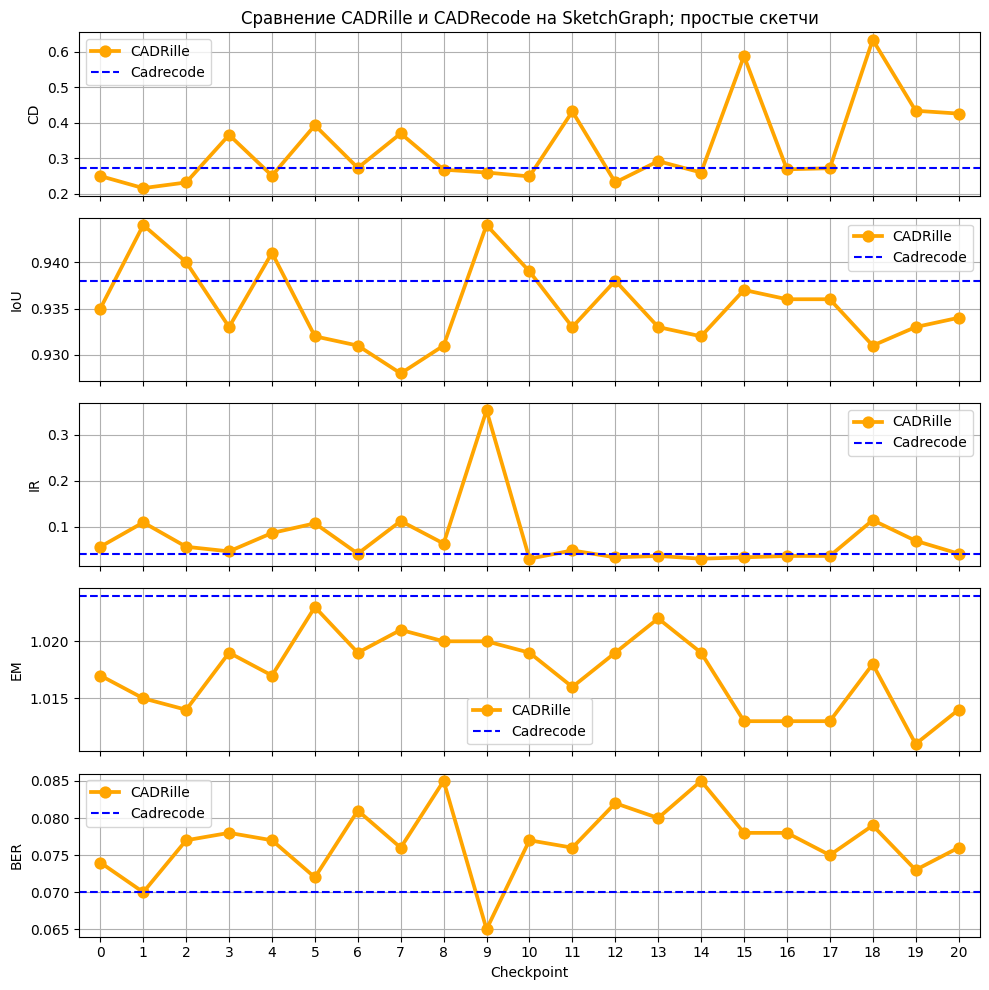
\includegraphics[width=\linewidth]{cadrille_sketchgraph_easy.png}
        \caption{Простые скетчи}
    \end{subfigure}

    \vspace{1em}

    \begin{subfigure}{0.4\linewidth}
        \centering
        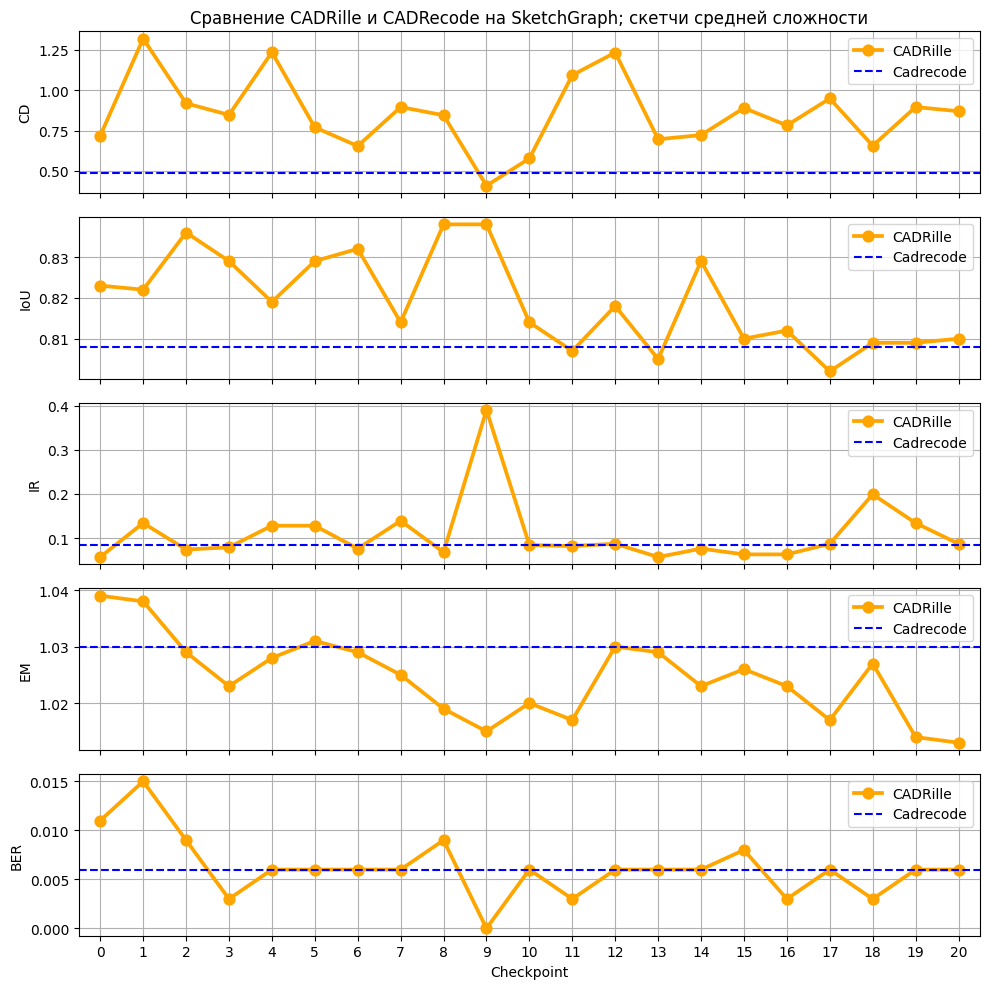
\includegraphics[width=\linewidth]{cadrille_sketchgraph_medium.png}
        \caption{Скетчи средней сложности}
    \end{subfigure}
    \hfill
    \begin{subfigure}{0.4\linewidth}
        \centering
        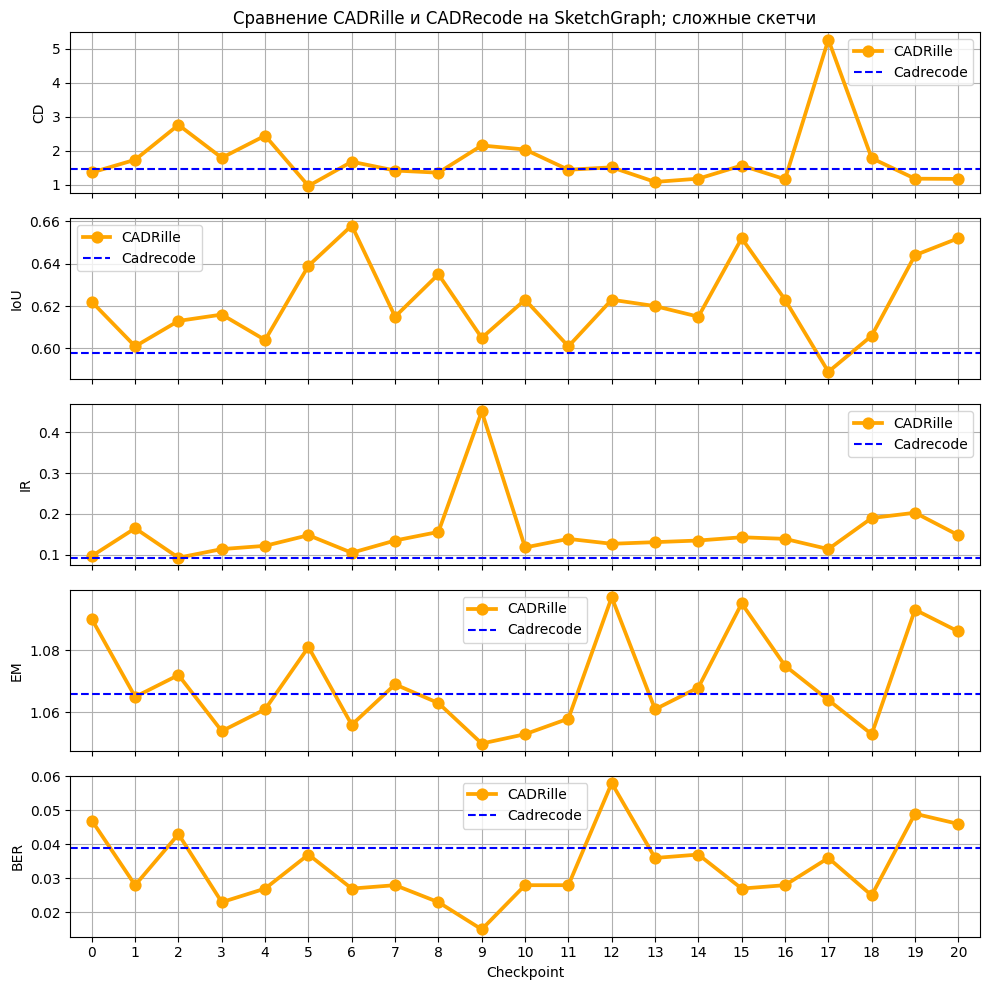
\includegraphics[width=\linewidth]{cadrille_sketchgraph_hard.png}
        \caption{Сложные скетчи}
    \end{subfigure}

    \caption{Результаты по метрикам CADRille с моделью CADRecode на SketchGraph и на трёх классах, разделённых по уровню сложности топологии.
        Верхняя диаграмма иллюстрирует метрику Chamfer Distance (CD), где меньшее значение лучше.
        Вторая диаграмма показывает Intersection over Union (IoU), где большее значение лучше.
        Третья диаграмма отражает показатель Invalid Rate (IR), где меньшее значение лучше.
        Метрики CD и IoU вычисляются только на валидных генерациях.
        EM (верхняя диаграмма) — это среднее число команд extrude (чем оно меньше, тем лучше).
        BER (нижняя диаграмма) — доля простейших макросов (cylinder или box) в среде CADQuery; желательно, чтобы это значение не было слишком высоким.}
    \label{fig:exp4}
\end{figure}

По результатам можно увидеть, что у CADRille растёт метрика IoU, а на скетчах лёгкого и среднего уровня наблюдается снижение количества команд \texttt{Extrude}.
Таким образом, подход CADRille не ухудшает способность CADRecode корректно рисовать скетчи, при этом повышая обобщающую способность модели.

\subsection{Синтетический датасет на SketchGraph.}
После интеграции скетчей из SketchGraph в пайплайн генератора CADRecode появилась возможность сгенерировать новый датасет и обучить на нём модель, сравнив результаты с датасетом на синтетических скетчах. Предполагается, что такой подход внесёт дополнительный индуктивный байас и улучшит метрики на всех датасетах.

Для эксперимента было сгенерировано два датасета на пайплайне генератора CADRecode~\cite{rukhovich24_cadrecode}, различающихся только типом скетчей. Обучение на каждом из них проходило на четырёх GPU H100 с размером батча 9 в течение 10 эпох. Время обучения обоих вариантов оказалось одинаковым.

\begin{figure}[h!]
    \centering
    \begin{subfigure}{0.45\linewidth}
        \centering
        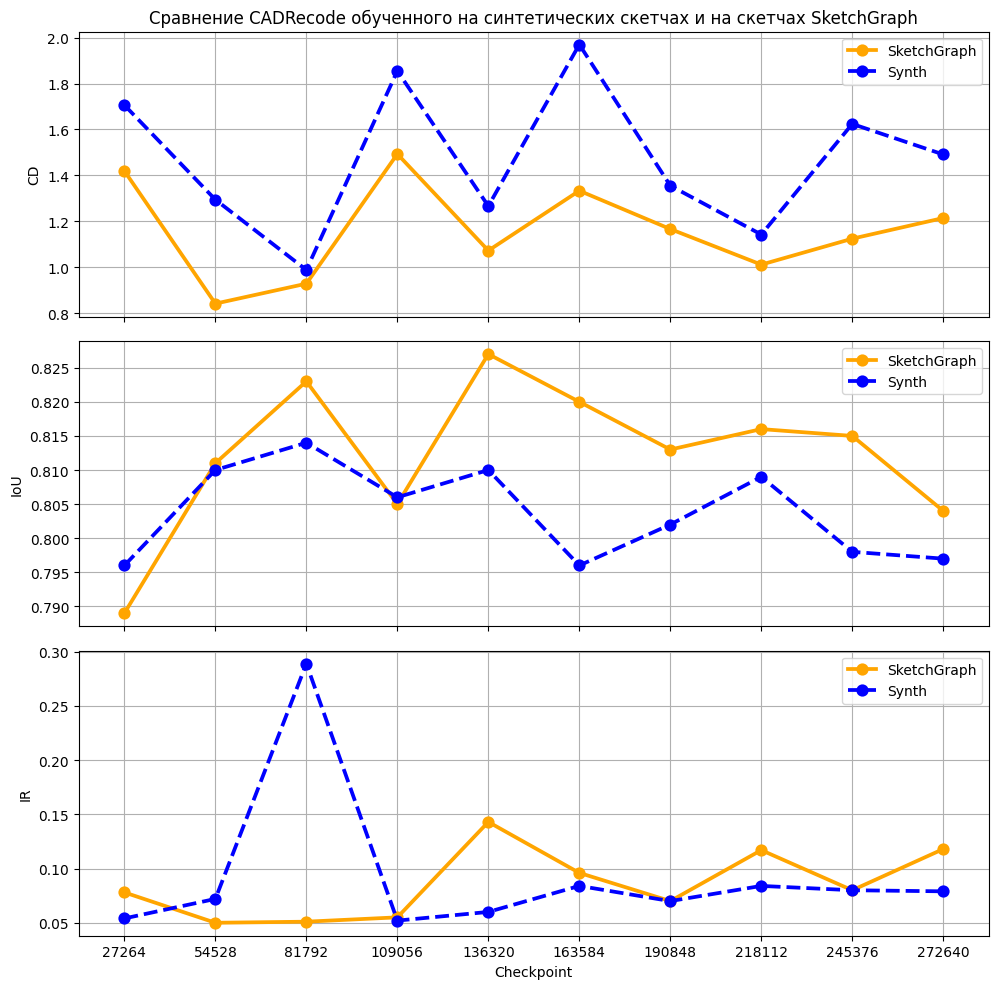
\includegraphics[width=\linewidth]{cadrecode_sg_deepcad.png}
        \caption{DeepCAD}
    \end{subfigure}
    \hfill
    \begin{subfigure}{0.45\linewidth}
        \centering
        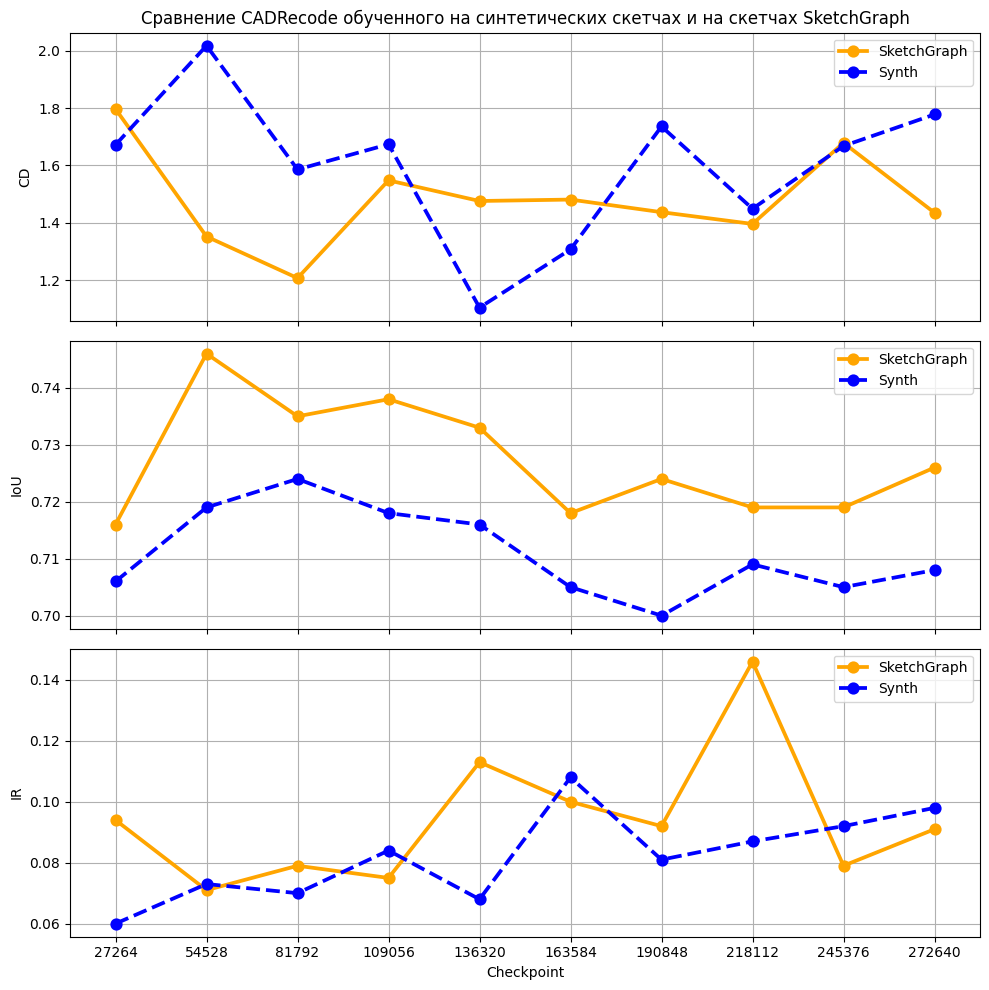
\includegraphics[width=\linewidth]{cadrecode_sg_fusion360.png}
        \caption{Fusion360}
    \end{subfigure}

    \vspace{1em}

    \begin{subfigure}{0.45\linewidth}
        \centering
        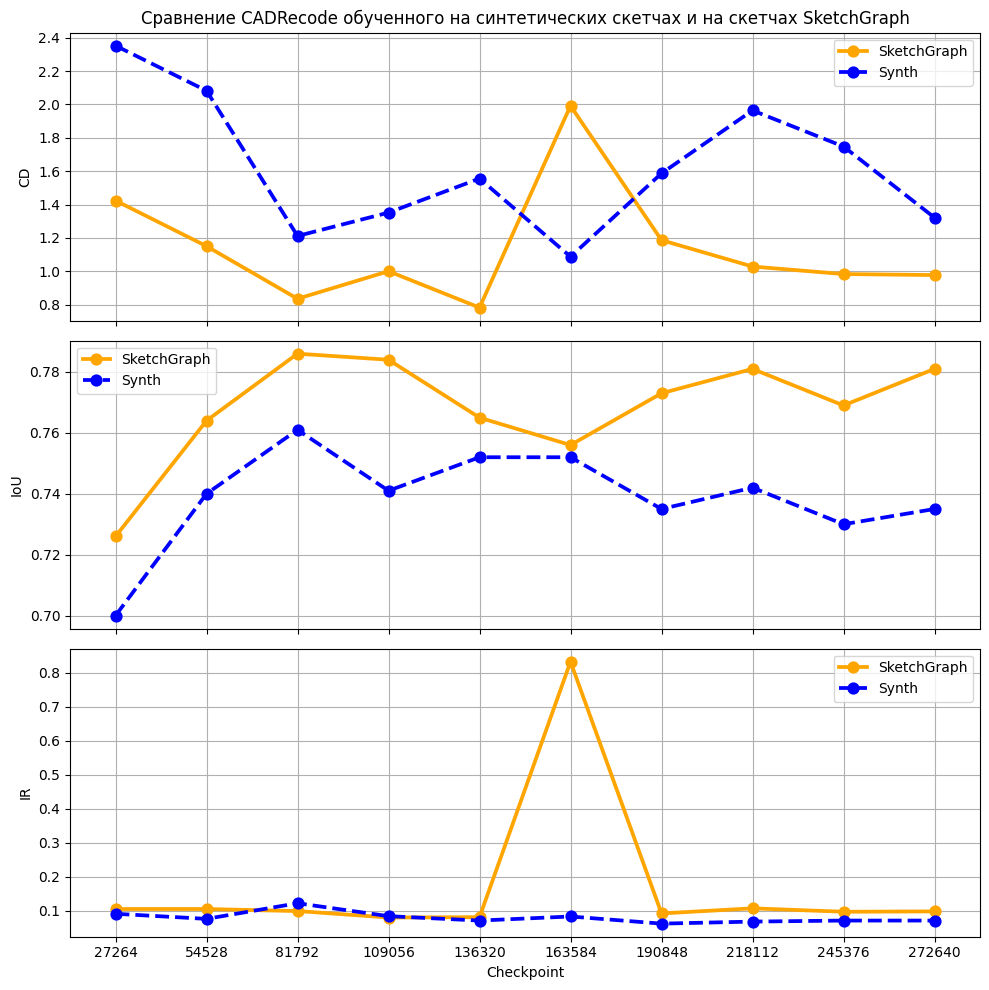
\includegraphics[width=\linewidth]{cadrecode_sg_sketchgraph.png}
        \caption{SketchGraph}
    \end{subfigure}
    \hfill
    \begin{subfigure}{0.45\linewidth}
        \centering
        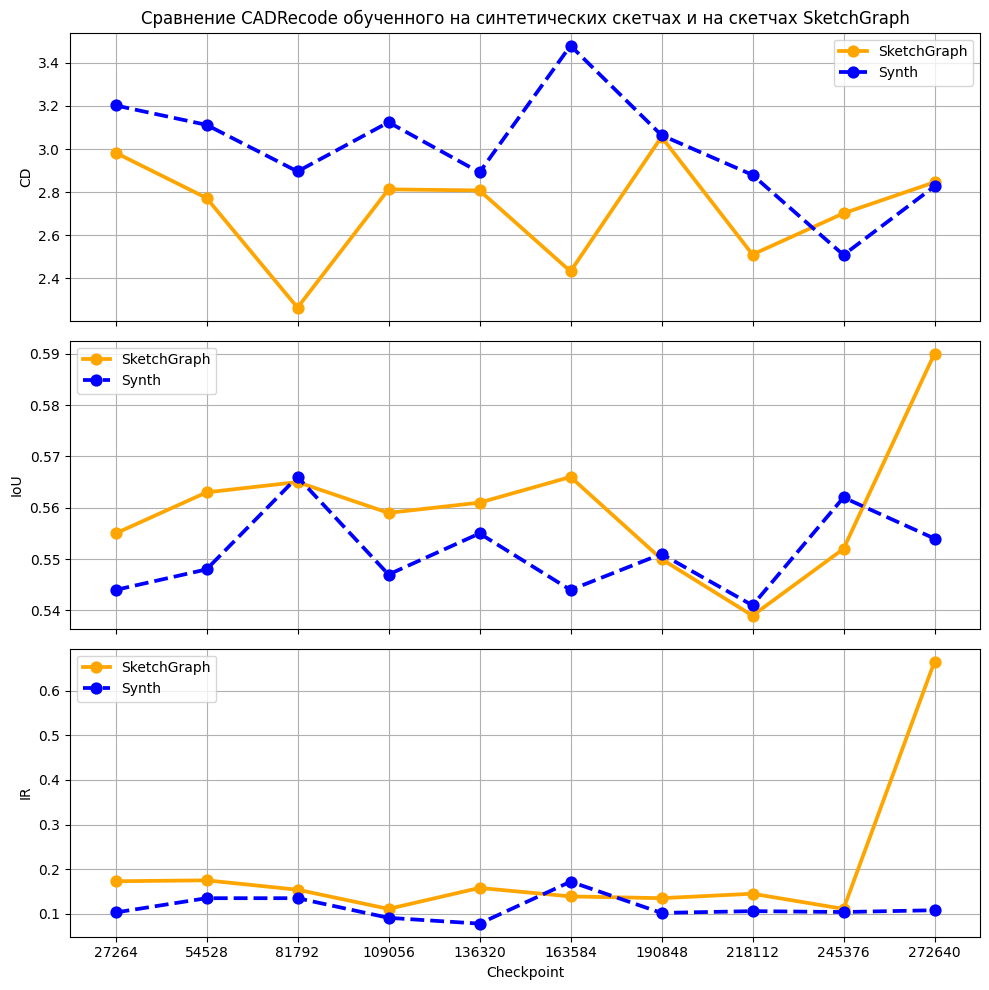
\includegraphics[width=\linewidth]{cadrecode_sg_cc3d.png}
        \caption{CC3D}
    \end{subfigure}

    \caption{Результаты экспериментов на DeepCAD, Fusion360, SketchGraph и CC3D.
        Верхний график показывает метрику Chamfer Distance (CD), где меньшие значения лучше.
        Второй график — Intersection over Union (IoU), где большие значения лучше.
        Последний график — Invalid Rate (IR), где меньшие значения лучше.
        CD и IoU подсчитаны только среди валидных генераций.}
    \label{fig:exp5}
\end{figure}

На рис.~\ref{fig:exp5} заметно, что модель, обученная на скетчах из SketchGraph, чаще демонстрирует более высокий IoU и меньший CD, что говорит об успешной интеграции данного подхода.
Сравним два лучших чекпоинта: модель на 81792-й итерации (скетчи из SketchGraph) и на 136320-й итерации (синтетические скетчи).

\begin{table}[h!]
    \centering
    \begin{tabular}{lccc}
        \toprule
        \textbf{Модель} & \textbf{CD}    & \textbf{IoU}   & \textbf{IR}    \\
        \midrule
        SketchGraph     & 1.207          & \textbf{0.735} & 0.079          \\
        Synth           & \textbf{1.104} & 0.716          & \textbf{0.068} \\
        \bottomrule
    \end{tabular}
    \caption{Результаты измерений на Fusion360.}
\end{table}

\begin{table}[h!]
    \centering
    \begin{tabular}{lccc}
        \toprule
        \textbf{Модель} & \textbf{CD}    & \textbf{IoU}   & \textbf{IR}    \\
        \midrule
        SketchGraph     & \textbf{0.928} & \textbf{0.823} & \textbf{0.051} \\
        Synth           & 1.266          & 0.810          & 0.060          \\
        \bottomrule
    \end{tabular}
    \caption{Результаты измерений на DeepCAD.}
\end{table}

\begin{table}[h!]
    \centering
    \begin{tabular}{lccc}
        \toprule
        \textbf{Модель} & \textbf{CD}    & \textbf{IoU}   & \textbf{IR}    \\
        \midrule
        SketchGraph     & \textbf{2.265} & \textbf{0.565} & 0.154          \\
        Synth           & 2.892          & 0.555          & \textbf{0.078} \\
        \bottomrule
    \end{tabular}
    \caption{Результаты измерений на CC3D.}
\end{table}

\begin{table}[h!]
    \centering
    \begin{tabular}{lccc}
        \toprule
        \textbf{Модель} & \textbf{CD}    & \textbf{IoU}   & \textbf{IR}    \\
        \midrule
        SketchGraph     & \textbf{0.836} & \textbf{0.786} & 0.099          \\
        Synth           & 1.556          & 0.752          & \textbf{0.071} \\
        \bottomrule
    \end{tabular}
    \caption{Результаты измерений на SketchGraph.}
\end{table}

Из таблиц видно, что модель, обученная на реальных скетчах, особенно хорошо проявляет себя на датасетах DeepCAD и SketchGraph. Вероятно, более сложные скетчи из Fusion360 и CC3D затрудняют процесс генерации, однако на DeepCAD и SketchGraph способность к более сложному рисованию становится ключевым фактором качества.

С другой стороны, на Fusion360 и CC3D нельзя однозначно утверждать превосходство одной модели над другой, в частности из-за отличий в Invalid Rate (IR).

Рассмотрим визуальное сравнение на датасете CC3D (рис.~\ref{fig:datasets1}).

\begin{figure}[h!]
    \centering
    
\includegraphics[width=\textwidth]{collage_with_gt_cc3d_synth.png}
    \caption*{Synth}
    \vspace{1em}
    
\includegraphics[width=\textwidth]{collage_with_gt_cc3d_sg.png}
    \caption*{SketchGraph}
    \caption{Визуальное сравнение результатов на CC3D.}
    \label{fig:datasets1}
\end{figure}

На данных примерах модель, обученная на реальных скетчах, лучше улавливает симметрию и демонстрирует аккуратные результаты, которые выглядят более редактируемыми.
В целом модель стала работать лучше, хотя систематически имеет более высокий Invalid Rate.
Вероятно, при применении RL-подхода (например, \texttt{CADRille}~\cite{kolodiazhnyi25_cadrille}) этот недостаток можно компенсировать и улучшить метрики ещё заметнее.

\subsection{Будущая работа}

В данной работе используется генератор CADRecode~\cite{rukhovich24_cadrecode}, однако я веду разработку собственного генератора, который будет ещё больше приближен к инженерным объектам за счёт новых правил построения.
К сожалению, на данный момент мой генератор имеет недоработки, из-за чего обучение не проходит успешно.

Также планируется внедрить изменения в архитектуру PointCloud-модуля в CADRecode, а именно протестировать на различных \textit{PointCloudEncoder} и подобрать оптимальное количество семплируемых точек для генерации.

Кроме того, планируется поставить эксперименты с RL-finetune на синтетике со скетчами SketchGraph, а также провести эксперименты с другой reward-функцией.

\newpage